\chapter{Fundamentos teóricos}

Este capítulo tiene el propósito de presentar y describir los fundamentos teóricos que sustentan los métodos 
utilizados en el trabajo, además de justificar su importtancia para abordar los problemas planteados.

% ------------------------------------------------------------------------------------------------------------
% MACHINE LEARNING -------------------------------------------------------------------------------------------
% ------------------------------------------------------------------------------------------------------------

\section{Machine Learning}

Frente a la idea de intentar crear un programa que simulara directamente el comportamiento inteligente de una 
``mente adulta'', Alan Turing ya vaticinó un enfoque alternativo \cite{turing1950}: que las máquinas pudieran 
aprender como lo hace un niño, mediante un ``proceso educativo'' con el cual se logra alcanzar progresivamente 
una ``mente adulta'', obteniendo así comportamientos inteligentes complejos.

En los años 50, surgió el concepto de \textit{machine learning} (ML) ---o aprendizaje automático en
español---, popularizado por Arthur L. Samuel \cite{samuel1959}, para designar una rama marginal de la IA, 
centrada en el desarrollo de modelos y algoritmos que permitiesen a las 
computadoras imitar la forma en la que los humanos aprenden, realizar tareas autónomas y mejorar su 
rendimiento a través de la experiencia y exposición a más datos. De esta forma, estos modelos podrían realizar 
predicciones o tomar decisiones sin ser programados para cada caso.

En las décadas de 1960, 1970 y 1980, surgieron algoritmos fundamentales como el perceptrón 
\cite{mcculloch1943,rosenblatt1958} o los árboles de decisión \cite{quinlan1986}, 
que sentaron los cimientos teóricos para el desarrollo posterior de técnicas más complejas.  
Sin embargo, el progreso fue lento debido a las limitaciones computacionales y el gran escepticismo académico. 

Los años 90 y 2000 marcaron un punto de inflexión para el ML, gracias a los avances teóricos, el mayor poder 
computacional y la disponibilidad de grandes volúmenes de datos. De 2010 en adelante, la evolución del ML ha 
sido exponencial, marcada por la consolidación del \textit{deep learning}, la escalabilidad masiva y su 
integración en numerosas aplicaciones: de visión por computador, reconocimiento de lenguaje natural, robótica, 
diagnóstico médico y forense, finanzas o recomendación de contenidos, entre otros. De esta forma, el ML se ha 
convertido en un campo tan amplio y exitoso que ahora ``eclipsa'' al resto de campos de la IA 
\cite{domingos2015}.

El ML diferencia tres tipos de aprendizaje en base a tres tipos de retroalimentación \cite{rusell2021}: 

\begin{itemize}
    
    \item \textbf{Aprendizaje supervisado}, en el que el agente (refiriéndose con este al modelo de ML y su 
    algoritmo de aprendizaje) observa ejemplos de pares entrada-salida y aprende la función que mejor mapea 
    las entradas (inputs) a las salidas (outputs) correspondientes. El objetivo es generalizar este 
    aprendizaje para hacer predicciones precisas sobre datos nuevos y no vistos \cite{bishop2006}.

    \item \textbf{Aprendizaje por refuerzo}, en el que los datos de entrenamiento no contienen salida 
    objetivo, sino que contiene posibles resultados junto con medidas de calidad de dicho resultado, es decir, 
    una función de evaluación del estado. En este tipo de aprendizaje, el agente toma decisiones en un entorno 
    y recibe recompensas o penalizaciones por las acciones que realiza, ajustando su comportamiento mediante 
    prueba y error, maximizando la recompensa acumulada en el tiempo \cite{alpaydin2010}.

    \item \textbf{Aprendizaje no supervisado}, en el que el agente tampoco dispone de valores de salida, solo 
    de entrada \cite{bishop2006}, y los objetivos pueden ser muy variados, centrándose en descubrir patrones, 
    estructuras o relaciones ocultas en los datos. A diferencia de los otros enfoques, aquí no hay una 
    ``respuesta correcta'' predefinida, sino que el modelo debe inferir conocimiento directamente desde la 
    distribución de los datos.

\end{itemize}

Este trabajo se centrará en el aprendizaje supervisado, pues es este tipo de aprendizaje el empleado en los 
problemas de clasificación y regresión que aplicaremos en el ámbito de la antropología forense.


% Retos en el aprendizaje supervisado


% No importa el formato de entrada



% ------------------------------------------------------------------------------------------------------------

% En el \textbf{aprendizaje supervisado} \cite{bishop2006}, el agente (refiriéndose con este al 
% modelo de ML y su algoritmo de aprendizaje) observa ejemplos de pares entrada-salida y aprende
% la función que mejor mapea las entradas (inputs) a las salidas (outputs) correspondientes. El 
% objetivo es generalizar este aprendizaje para hacer predicciones precisas sobre datos nuevos y 
% no vistos.

% Hay dos principales tipos de problemas de aprendizaje supervisado: 

% \begin{itemize}
%     \item la \textit{clasificación} para cuando el valor de salida es una etiqueta categórica, y
%     \item la \textit{regresión} cuando el valor de salida es un valor continuo.
% \end{itemize}

% % ----------------------------------------------------------------------------------------------------------

% En cambio, en el \textbf{aprendizaje por refuerzo}, los datos de entrenamiento no contienen 
% salida objetivo, sino que contiene posibles resultados junto con medidas de calidad de dicho 
% resultado, es decir, una función de evaluación del estado. En este tipo de aprendizaje, el 
% agente toma decisiones en un entorno y recibe recompensas o penalizaciones por las acciones 
% que realiza, ajustando su comportamiento mediante prueba y error, maximizando la recompensa 
% acumulada en el tiempo \cite{alpaydin2010}.  

% De esta forma, el algoritmo no aprende a dar una acción/salida a partir de un input, sino que 
% desarrolla una política que determina la mejor acción a tomar en cada estado del entorno, con 
% el objetivo de maximizar la recompensa acumulada a largo plazo.

% Esta aproximación es clave en aplicaciones como juegos, robótica, optimización de recursos y 
% sistemas conversacionales (ChatAI), donde las decisiones secuenciales y la interacción 
% dinámica con el entorno son fundamentales.

% % ----------------------------------------------------------------------------------------------------------

% Y, por último, en el \textbf{aprendizaje no supervisado}, el agente tampoco dispone de valores 
% de salida, solo de entrada \cite{bishop2006}, y los objetivos pueden ser muy variados, 
% centrándose en descubrir patrones, estructuras o relaciones ocultas en los datos. 

% A diferencia de los otros enfoques, aquí no hay una "respuesta correcta" predefinida, sino que 
% el modelo debe inferir conocimiento directamente desde la distribución de los datos.

% Algunos problemas clásicos de este tipo de aprendizaje son: 

% \begin{itemize}

%     \item El \textit{clustering} o agrupamiento, donde el objetivo es encontrar clústeres o 
%     agrupaciones del input. Esto puede ser útil, por ejemplo, para una empresa que quiera 
%     segmentar sus clientes, o para identificar patrones en datos genéticos sin etiquetar.
    
%     \item La \textit{detección de anomalías} (\textit{outlier detection} en inglés), que 
%     consiste en encontrar instancias atípicas o inusuales en los datos. Sus aplicaciones 
%     incluyen: identificación de fraudes en transacciones bancarias, fallos en equipos 
%     industriales o identificación de ciberataques.

%     \item La \textit{reducción de dimensionalidad}, que trata de reducir el número de 
%     variables manteniendo la mayor información posible. Esto es útil para visualizar datos 
%     complejos o mejorar la eficiencia de algoritmos (p.ej., transformaciones PCA y t-SNE).

%     \item El \textit{aprendizaje de representaciones} (como los \textit{autoencoders}), 
%     donde el modelo busca capturar características latentes de los datos de manera eficiente. 
%     La compresión de archivos o la reducción de ruido en imágenes son algunos ejemplos de 
%     aplicaciones. 

% \end{itemize}



% ------------------------------------------------------------------------------------------------------------

\subsection{Problemas de regresión}

Como se ha mencionado antes, la regresión es un tipo de problema clásico en el aprendizaje supervisado, y 
consiste en predecir el valor de una o más \textbf{variables continuas} objetivo a partir de unos datos de 
entrada \cite{bishop2006}, utilizando un modelo entrenado con ejemplos ya con valores conocidos.

Matemáticamente, este proceso implica modelar la relación entre la variable dependiente $Y$ y las variables
independientes $X$, de modo que se pueda predecir o explicar el comportamiento de $Y$ en función de los 
valores de $X$. El modelo aprende una función de predicción $f$ que, dado un nuevo ejemplo $i$ con 
características $X_i$, genera una estimación $\hat{Y_i}$:

$$
f(X_i) = f(X_{i0}, X_{i1}, \dots, X_{in}) = \hat{Y_i} = Y_i + \varepsilon_i
$$

donde 

\begin{itemize}
    \item $X_{i0},X_{i1}, \dots, X_{in}$ son las características o atributos del ejemplo $i$,
    \item $Y_i$ es el valor real de la variable objetivo para ese ejemplo,
    \item $\hat{Y_i}$ es la predicción generada por el modelo, y
    \item $\varepsilon_i$ representa el error o residuo 
    \footnote{
        ... a pesar de que en la literatura estos términos se distinguen, ...
    }, 
    es decir, la diferencia entre la predicción y el valor real.
    Este término captura factores aleatorios o imprecisiones que el modelo no logra explicar perfectamente.
\end{itemize}

El análisis y la evaluación estadística del error son fundamentales para valorar la utilidad práctica del 
modelo y optimizar su capacidad predictiva mediante técnicas de ajuste y validación. Existen numerosas 
métricas para evaluar el rendimiento en problemas de regresión, pero tres destacan especialmente por ser 
\textit{model-agnostic}, es decir, aplicables a cualquier modelo de regresión independientemente del algoritmo 
subyacente. Estas son:

\begin{itemize}
    \item El \textbf{error absoluto medio (\textit{mean absolute error}, MAE)} mide el promedio de las 
    diferencias absolutas entre los valores reales ($Y_i$) y los valores predichos ($\hat{Y_i}$) por el 
    modelo.

    $$
    MAE = \frac{1}{n} \sum_{i=1}^n{|Y_i - \hat{Y_i}|}
    $$

    donde $n$ es el número de ejemplos/instancias con las que se cuenta en los datos a evaluar.

    La interpretación más inmediata de esta métrica es que representa cuánto se desvía en promedio la 
    predicción del valor real sin considerar la dirección del error (positivo o negativo) y, por tanto, cuanto 
    más se acerque a cero el valor, mejor es el ajuste del modelo.

    Existe una variante denominada \textbf{error absoluto mediano (\textit{median absolute error}, MedAE)}, 
    que realiza la mediana de las diferencias absolutas, en vez de la media, aumentando la robustez frente a 
    valores atípicos con errores extremos.

    \item El \textbf{error cuadrático medio (\textit{mean squared error}, MSE)} mide el promedio de los 
    errores al cuadrado entre valores reales ($Y_i$) y los valores predichos ($\hat{Y_i}$) por el modelo.
    
    $$
    MSE = \frac{1}{n} \sum_{i=1}^n{(Y_i - \hat{Y_i})^2}
    $$

    Al igual que el MAE, cuantifica qué tan cerca están las predicciones de los valores reales, pero penaliza
    más los errores grandes, y es más sensible por tanto a valores atípicos.

    Como veremos más tarde, esta métrica es muy útil en optimización mediante gradiente descendente, usado a 
    la hora de entrenar modelos de regresión basados en redes neuronales.

    Y también tiene una variante, la \textbf{raíz del error cuadrático medio (\textit{root mean square error}, 
    RMSE)}, que se obtiene extrayendo la raíz cuadrada del MSE:

    $$
    RMSE = \sqrt{\frac{1}{n} \sum_{i=1}^{n}{(Y_i-\hat{Y_i})^2} }
    $$

    Esta métrica conserva las mismas unidades que la variable objetivo, lo que facilita su interpretación 
    práctica. Es comparable con el MAE en cuanto a escala, aunque sigue penalizando más los errores grandes.

    \item El \textbf{coeficiente de determinación}, o más conocido como \textbf{R² o bondad de ajuste}, mide 
    la proporción de la variabilidad de la variable dependiente ($Y$) que es explicada por el modelo.

    $$
    R^2 = 1 - \frac{\sum_{i=1}^n (Y_i - \hat{Y}_i)^2}{\sum_{i=1}^n (Y_i - \bar{Y})^2}
    $$

    donde 

    \begin{itemize}

        \item $Y_i$ es el valor real de la variable dependiente para la instancia $i$,
        
        \item $\hat{Y_i}$ es la predicción generada por el modelo, y
        
        \item $\bar{Y}$ es el promedio de los valores reales de la variable dependiente a lo largo de todas 
        las instancias del conjunto de datos.
    
    \end{itemize}
    

    El valor de esta métrica varía entre $-\infty$ y 1, y su interpretación es la siguiente:

    \begin{itemize}

        \item $R^2 \le 0$ significa que el modelo no explica ninguna variabilidad y que las predicciones del 
        modelo no son mejores que simplemente predecir la media de los valores reales.
        
        \item $R^2 \in \left(0,1\right)$ indica que el modelo está explicando una fracción de la variabilidad 
        de los datos, y cuanto más cercano sea a 1, mejor será el ajuste del modelo.
        
        \item $R^2 = 1$ indica un ajuste perfecto y, por tanto, el modelo explica toda la variabilidad de los 
        datos. 
    
    \end{itemize}

    A diferencia de las anteriores, es una métrica relativa y adimensional, es decir, no depende de las 
    unidades de la variable objetivo y evalúa qué tan bien se ajusta el modelo en comparación con un modelo 
    base que siempre predice la media de los valores reales.
    
\end{itemize}

% Elementos visuales

No obstante, el uso exclusivo de métricas numéricas resulta en un análisis pobre, ya que estas no permiten 
identificar patrones ocultos, detectar relaciones no lineales ni distinguir entre errores positivos o 
negativos. Por esta razón, se recomienda completar el análisis con representaciones gráficas, tales como:

\begin{itemize}

    \item La \textbf{gráfica de puntos de valores reales vs. predichos}, que permite visualizar la relación 
    entre las predicciones del modelo y los valores reales. Idealmente, los puntos deberían alinearse 
    alrededor de la recta $Y=\hat{Y}$. Desviaciones sistemáticas indican sesgos o problemas de ajuste. Un 
    ejemplo de esta gráfica lo encontramos en la Figura \ref{fig:scatter_pred_vs_act_AE}.

    \begin{figure}[h]
        \centering
        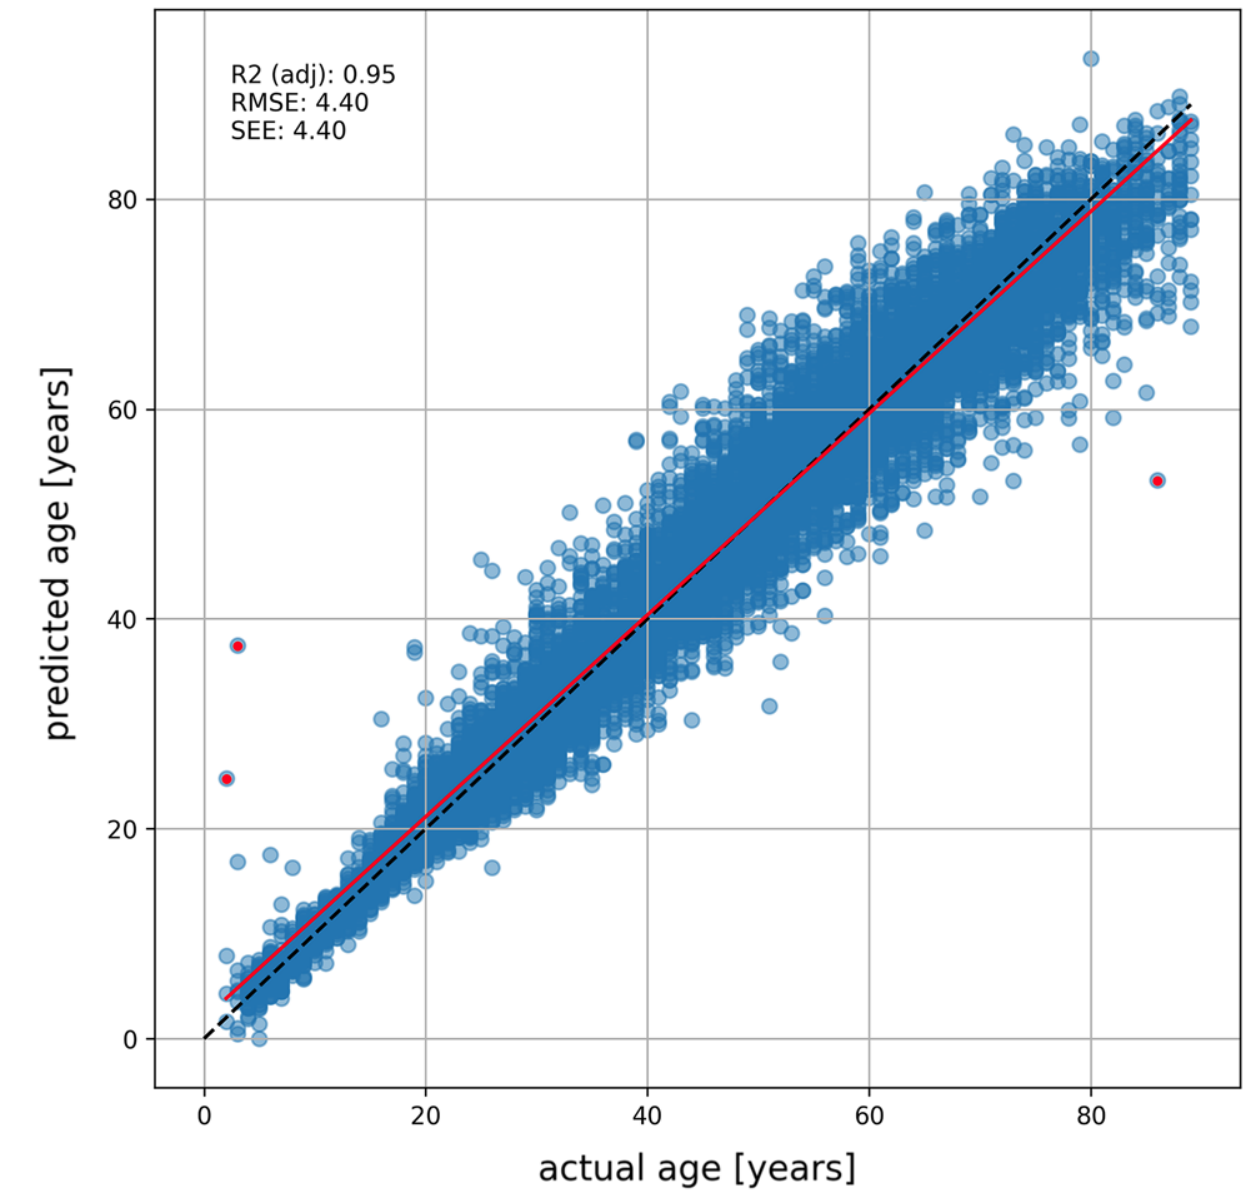
\includegraphics[width=0.5\textwidth]{capitulos/cap_02/imagenes/scatterplot_pred_vs_act_AE.png}
        \caption[
            Gráfica de puntos de valores de edad reales vs. predichos obtenidos por el modelo propuesto 
            en \cite{heinrich2024}.
        ]{
            Gráfica de puntos de valores de edad reales vs. predichos obtenidos por el modelo propuesto 
            en \cite{heinrich2024}. Se observan valores más dispersos en edades avanzadas.
        } 
        \label{fig:scatter_pred_vs_act_AE}
    \end{figure}

    \item También existe una versión más refinada de presentar esta información, especialmente útil en casos 
    en los que muchos datos sobrecargan la gráfica, en \textbf{la gráfica de cajas (en inglés 
    \textit{boxplot}) de valores reales vs. predichos}. Estos proporcionan una visión clara de la distribución 
    de los datos, con mediana, cuartiles y valores atípicos, ya sea agrupando por valores reales o por valores 
    predichos.

    La Figura \ref{fig:boxplot_pred_vs_act_AE} muestra la distribución de las edades predichas en función de 
    distintos grupos de edad real, y viceversa, lo que facilita la identificación de errores en el desempeño 
    del modelo.

    \begin{figure}[h]
        \centering
    
        \begin{subfigure}[b]{0.45\textwidth}
            \centering
            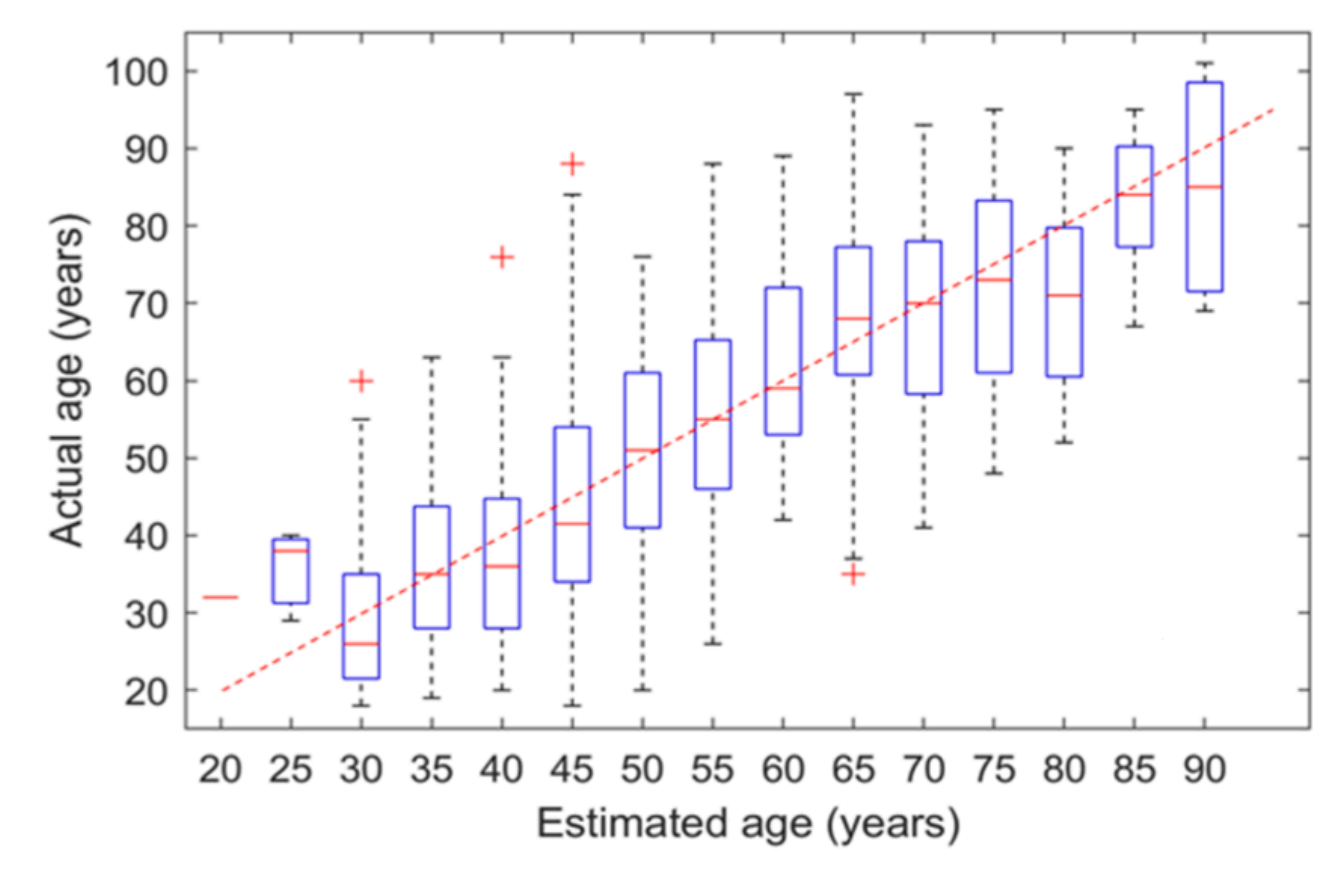
\includegraphics[width=\textwidth]{capitulos/cap_02/imagenes/boxplot_pred_vs_act_AE_1.png}
            \caption{Gráfica de cajas de edades reales en función de la estimada}
            \label{fig:boxplot_pred_vs_act_AE_a}
        \end{subfigure}
        \hfill
        \begin{subfigure}[b]{0.45\textwidth}
            \centering
            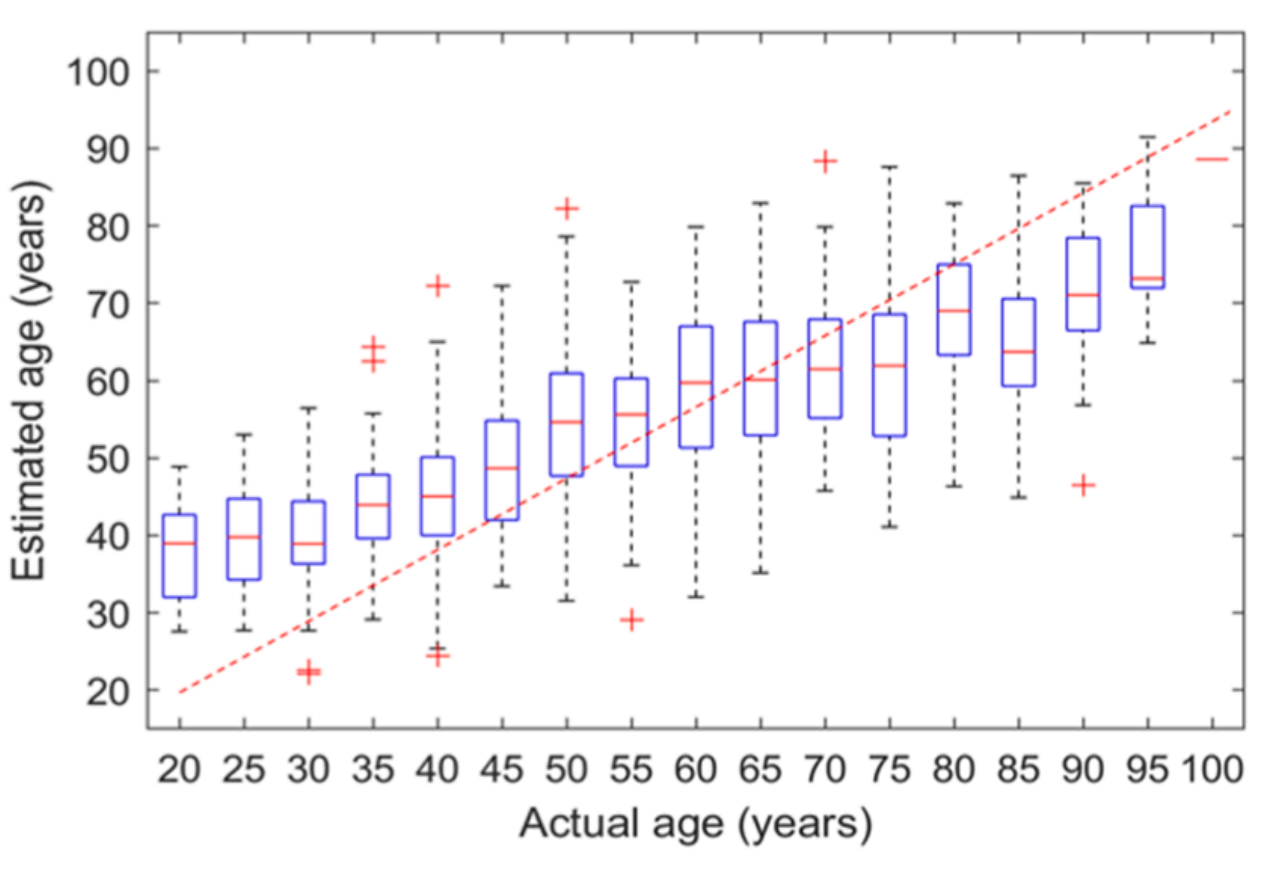
\includegraphics[width=\textwidth]{capitulos/cap_02/imagenes/boxplot_pred_vs_act_AE_2.png}
            \caption{Gráfica de cajas de edades estimadas en función de la real}
            \label{fig:boxplot_pred_vs_act_AE_b}
        \end{subfigure}
    
        \caption[
            Gráfica de cajas de valores de edad reales vs. predichos obtenidos por el modelo propuesto en 
            \cite{stepanovsky2024}.
        ]{
            Gráfica de cajas de valores de edad reales vs. predichos obtenidos por el modelo propuesto en 
            \cite{stepanovsky2024}. Se observa en \ref{sub@fig:boxplot_pred_vs_act_AE_b} que se sobreestima 
            la edad en personas jóvenes y se subestima 
            en personas de edad avanzada.
        }
        \label{fig:boxplot_pred_vs_act_AE}
    \end{figure}

    \item El \textbf{histograma de residuos} muestra la distribución de los errores (\(Y_i - \hat{Y}_i\)) del 
    modelo. Una distribución simétrica y centrada en cero sugiere un buen ajuste, mientras que una 
    distribución sesgada o asimétrica podría indicar que el modelo está subajustado o que hay algún patrón no 
    capturado por el modelo. 

    Un ejemplo de este tipo de gráfica lo encontramos en la Figura \ref{fig:prob_dist_AEerror}, donde se 
    analizaba el error obtenido con el modelo propuesto en \cite{stepanovsky2024}.

    Histograma de errores residuales del modelo de regresión propuesto en \cite{verma2020} que predice la 
    estatura a partir de la longitud de la tibia.

    \begin{figure}[h]
        \centering
        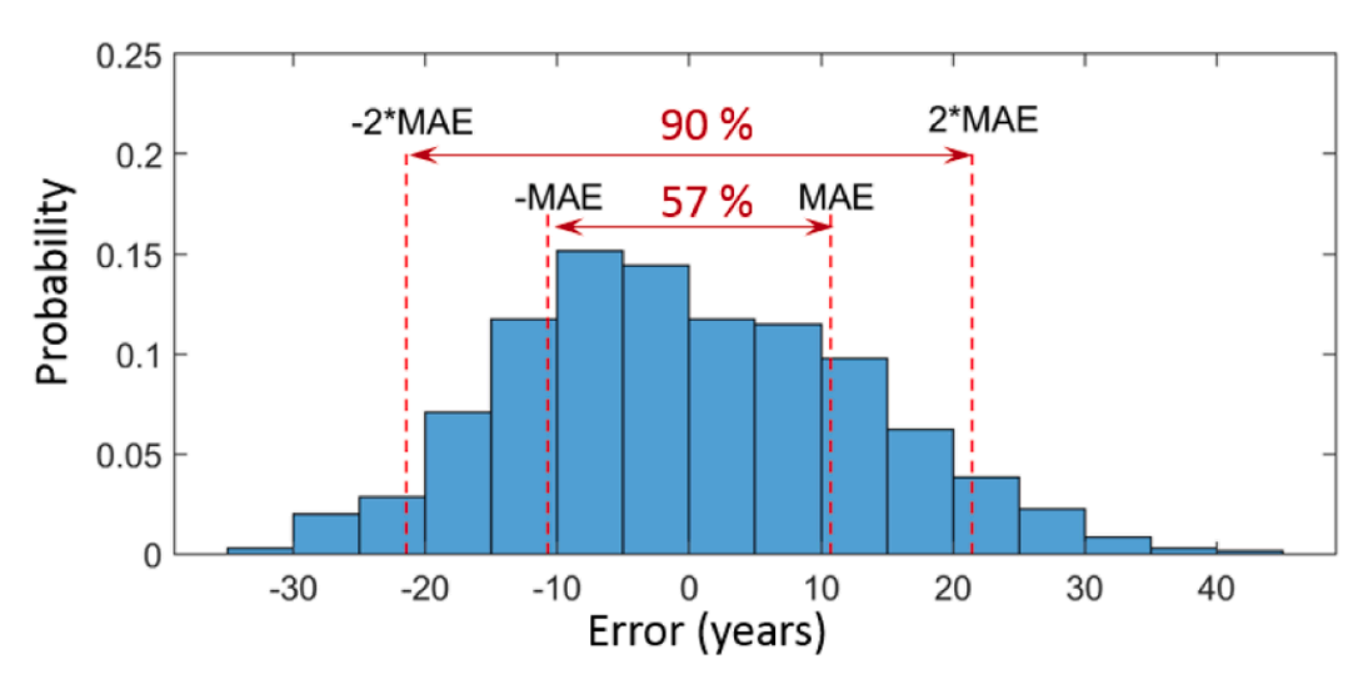
\includegraphics[width=0.8\textwidth]{capitulos/cap_02/imagenes/prob_distribution_AEerror.png}
        \caption[
            Histograma de errores residuales del modelo de estimación de edad propuesto en 
            \cite{stepanovsky2024}.
        ]{
            Histograma de errores residuales del modelo de estimación de edad propuesto en 
            \cite{stepanovsky2024}. Se evidencia una mayor probabilidad de errores negativos 
            (infraestimaciones) en comparación con los positivos Además, se destaca que el 57\% de las 
            predicciones presentan un error inferior al $\textnormal{MAE}$, y que el 90\% se encuentra dentro 
            de un margen de error menor a $2\textnormal{MAE}$.
        } 
        \label{fig:prob_dist_AEerror}
    \end{figure}


    \item Y una versión más completa que este último es la \textbf{gráfica de cajas de la distribución del 
    error en base a los valores reales o predichos}, que permite analizar cómo varía el error del modelo a lo 
    largo de diferentes rangos de valores, ya sean reales o predichos. Estas visualizaciones nos permiten 
    detectar fácilmente las fortalezas y debilidades en las predicciones del modelo, así como diagnosticar 
    sesgo o insuficiencia de datos en ciertas categorías.
    
    Un ejemplo ilustrativo de esta gráfica se presenta en la Figura \ref{fig:boxplot_error_vs_act_AE}, donde 
    se observa la variación del error del modelo propuesto en \cite{heinrich2024} a través de distintos rangos 
    de edad real. En particular, se evidencia una tendencia a cometer errores mayores en los grupos de edad 
    más avanzada.

    \begin{figure}[h]
        \centering
        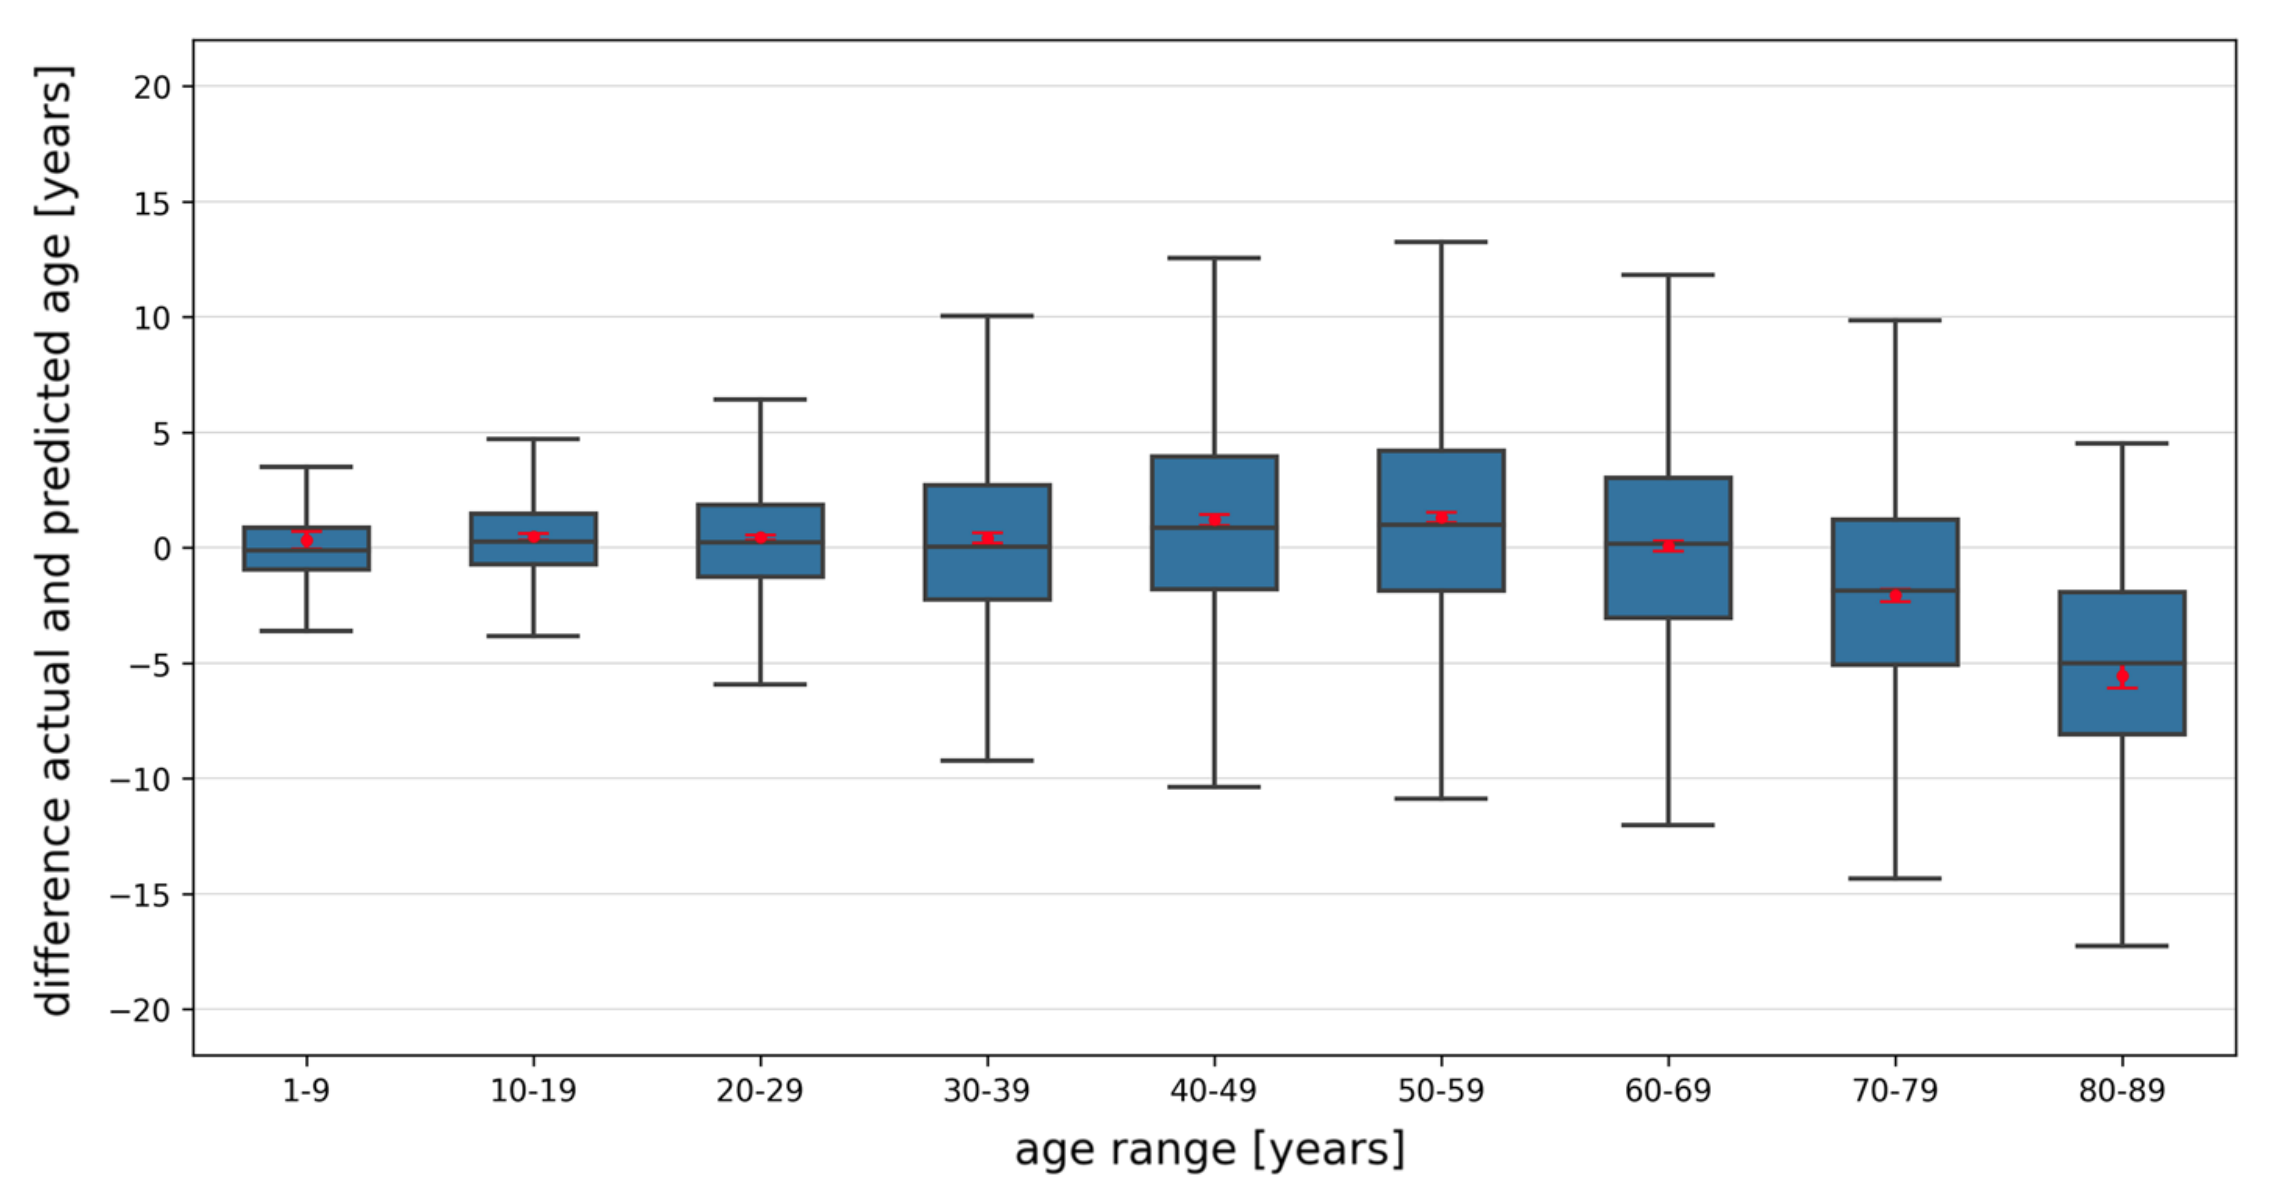
\includegraphics[width=0.95\textwidth]{capitulos/cap_02/imagenes/boxplot_error_vs_act_AE.png}
        \caption{
            Gráfica de cajas de la distribución del error de estimación de edad en función de la edad 
            real, obtenida en el modelo propuesto en \cite{heinrich2024}.
        } 
        \label{fig:boxplot_error_vs_act_AE}
    \end{figure}

\end{itemize}






% ------------------------------------------------------------------------------------------------------------

\subsection{Problemas de clasificación}

En cambio, en los problemas de clasificación, los valores de salida son categóricos, denominados más 
comúnmente como \textbf{clases}, y a cada valor individual asignado a una instancia de datos se le conoce como 
\textbf{etiqueta} (\textit{label} en inglés).

Existen multitud de variante de clasificación, que pueden diferenciarse según diversos criterios:

\begin{itemize}
    \item En base a la cardinalidad de las clases de salida: \textbf{clasificación binaria o multiclase}, 
    según si existen dos clases posibles o más de dos, respectivamente.

    \item En base al número de etiquetas asignadas a cada instancia: \textbf{clasificación con etiqueta única 
    o multietiqueta}, según si cada instancia pertenece a una sola clase o a varias de forma simultánea.

    \item En base a la certeza de la asignación de clases: \textbf{clasificación con etiqueta precisa o 
    difusa}, donde en el primer caso la asignación a una clase es determinista, y en el segundo caso se 
    permite una pertenencia parcial a varias clases, con distinto grados de afinidad.
    
\end{itemize}

No obstante, la mayoría de los problemas estudiados en la literatura de ML, y concretamente en antropología 
forense, corresponden a clasificación binaria o multiclase, con etiquetas únicas y asignación precisa 
\cite{bishop2006}, que serán el foco de este trabajo. La cardinalidad de las clases tiene implicanciones 
significativas en el diseño del modelo y la evaluación de su desempeño:

\begin{itemize}

    \item \textbf{Clasificación binaria}, que es aquella en la que existen únicamente dos clases posibles para 
    la variable objetivo, siendo común en problemas donde se desea discriminar entre dos estados mutuamente 
    excluyentes (p.ej., ``positivo'' vs. ``negativo'', ``spam'' vs. ``no spam'', ``fraude'' vs. ``no 
    fraude'').
    
    Se suele denominar a una de las clases como ``positiva'' y a otra como ``negativa'' para facilitar la 
    interpretación de métricas como la precisión, la sensibilidad o la especifidad, si bien no tiene por qué 
    existir una connotación valorativa entre ambas clases.
    
    \item \textbf{Clasificación multiclase}: en este caso, la variable objetivo puede tomar más de dos valores 
    posibles, pertenecientes a un conjunto finito. Un ejemplo de problema clásico es el de clasificar dígitos
    manuscritos (0-9).

\end{itemize}

En este tipo de problemas, el error ocurre cuando no se acierta al predecir la clase del ejemplo.

% Tanto en clasificación binaria como multiclase, un problema común es el desequilibrio de clases, donde una 
% clase tiene muchos más ejemplos que otra. Esto afecta el entrenamiento del modelo, ya que puede sesgarse 
% hacia la clase mayoritaria, ya que el modelo


Una vez definido los tipo de problemas de clasificación, es fundamental establecer cómo medir la efectividad 
del modelo predictivo. A continuación, se detallan los principales criterios y elementos gráficos utilizados 
para evaluar y comparar modelos de clasificación:

\begin{itemize}
    
    \item La \textbf{matriz de confusión} es una herramienta fundamental que permite visualizar el rendimiento 
    de modelos de clasificación, tanto binarios como multiclase. Esta muestra una tabla con tantas columnas y 
    filas como clases haya. En un eje, se representan las clases reales (etiquetas verdaderas), y en el otro 
    eje, las clases predichas por el modelo. Cada celda de la matriz indica la cantidad de ejemplos que 
    pertenecen a una clase real específica y que han sido clasificados como una clase predicha específica 
    (véase la Figura \ref{fig:conf_matrix_binary}).

    Idealmente, los valores se concentrarían en la diagonal principal, lo que indicaría que las predicciones 
    coinciden con los valores reales.

    \begin{figure}[h]
        \centering
        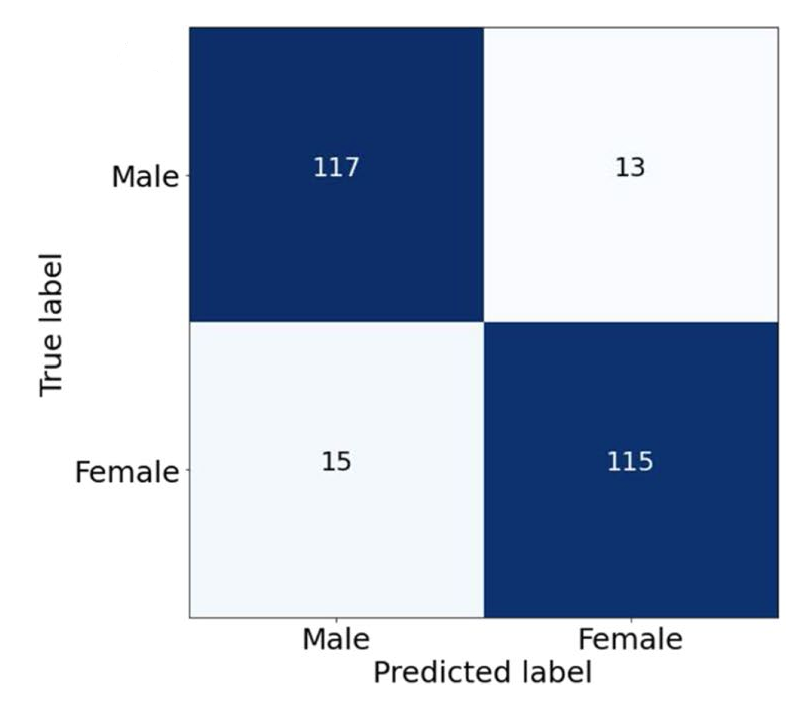
\includegraphics[width=0.6\textwidth]{capitulos/cap_02/imagenes/confusion_matrix_binary.png}
        \caption{
            Matriz de confusión para la estimación de sexo según el modelo \textit{random forest} 
            propuesto en \cite{bidmos2023}.
        } 
        \label{fig:conf_matrix_binary}
    \end{figure}

    Esta visualización admite muchas variantes, por ejemplo, como la vista en la Figura 
    \ref{fig:conf_matrix_binary_relative}.
    
    \begin{figure}[h]
        \centering
    
        \begin{subfigure}[b]{0.3\textwidth}
            \centering
            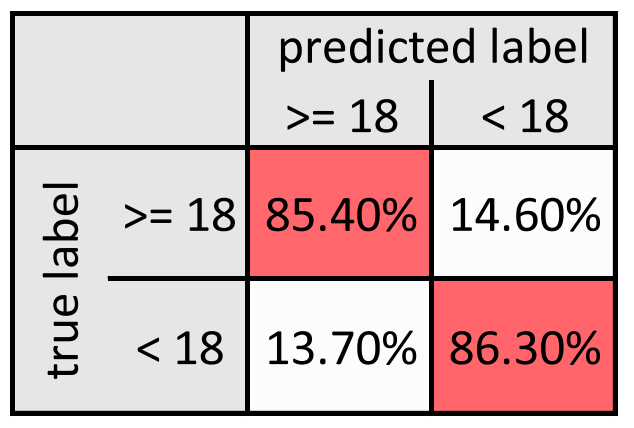
\includegraphics[width=\textwidth]{capitulos/cap_02/imagenes/confusion_matrix_binary_1.png}
            \caption{Sin información de sexo}
            \label{fig:conf_matrix_general}
        \end{subfigure}
        \hfill
        \begin{subfigure}[b]{0.3\textwidth}
            \centering
            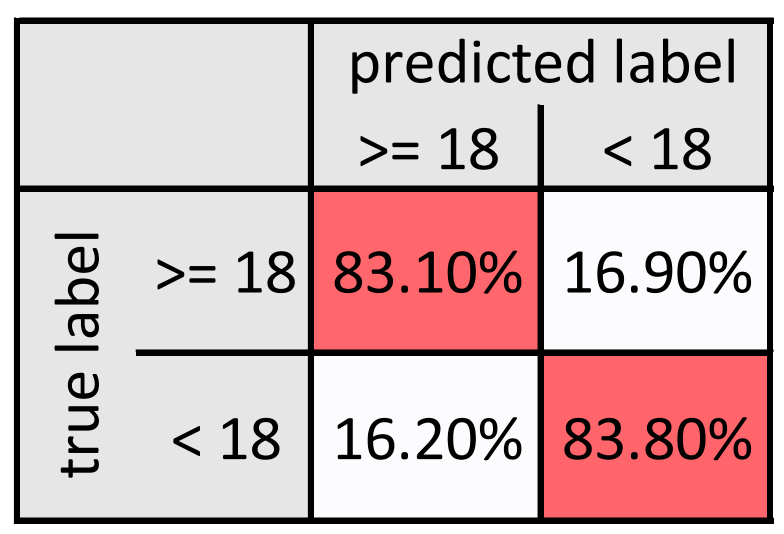
\includegraphics[width=\textwidth]{capitulos/cap_02/imagenes/confusion_matrix_binary_2.png}
            \caption{Sexo femenino}
            \label{fig:conf_matrix_female}
        \end{subfigure}
        \hfill
        \begin{subfigure}[b]{0.3\textwidth}
            \centering
            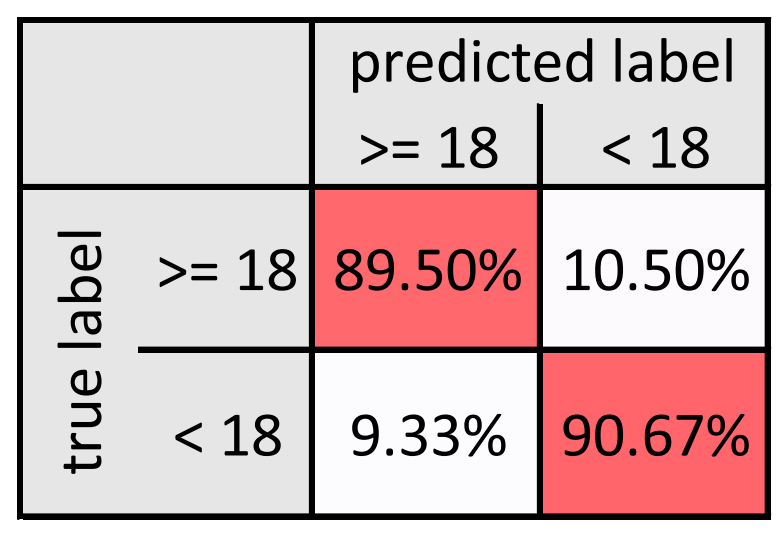
\includegraphics[width=\textwidth]{capitulos/cap_02/imagenes/confusion_matrix_binary_3.png}
            \caption{Sexo masculino}
            \label{fig:conf_matrix_male}
        \end{subfigure}
    
        \caption[
            Matrices de confusión para la estimación de mayoría/minoría de edad según el modelo de 
            \cite{porto2020}.
        ]{
            Matrices de confusión para la estimación de mayoría/minoría de edad según el modelo de 
            \cite{porto2020}.
            Se representan los valores de cada celda en términos porcentuales de los ejemplos reales que hay 
            de cada clase ($< 18$ y $\ge 18$), lo que permite comparar la matriz de confusión general de todos 
            los ejemplos (\ref{sub@fig:conf_matrix_general}) con la de ejemplos se sexo femenino 
            (\ref{sub@fig:conf_matrix_female}) y sexo masculino (\ref{sub@fig:conf_matrix_male}), permitiendo 
            identificar posibles sesgos en el modelo respecto al género, y así realizar una evaluación más 
            precisa del rendimiento del modelo en diferentes subgrupos de la población.
        }
        \label{fig:conf_matrix_binary_relative}
    \end{figure}

    Prácticamente todas las métricas y visualizaciones parten de la información ofrecida en esta matriz. 
    

    \item La \textbf{exactitud (\textit{accuracy})} es la proporción de predicciones correctas sobre el total.
    En clasificación binaria esto sería:
    
    $$
    \textnormal{Accuracy} = \frac{TP+TN}{TP+TN+FP+FN}
    $$

    En el caso de clasificación multiclase, esta se generaliza como:

    $$
    \textnormal{Accuracy} = 
        \frac{\textnormal{Numero de predicciones correctas}}{\textnormal{Número total de ejemplos}} =
        \frac{1}{N} \sum_{i=1}^N1(\hat{y_i}=y_i)
    $$

    donde $\hat{y_i}$ es la etiqueta predicha, $y_i$ la etiqueta verdadera para el ejemplo $i$, $N$ es el 
    número de ejemplos, y 1 es la función indicadora, que vale 1 si la predicción es correcta y 0 si no 
    lo es. 

    Los valores de esta métrica varían entre 0 y 1, donde 0 es el peor desempeño posible (todas las 
    predicciones son incorrectas) y 1 es el mejor desempeño posible (todas las predicciones son correctas).

    Es la medida más intuitiva, si bien puede dar una falsa impresión de buen desempeño si las clases 
    mayoritarias dominan la métrica. Es por esto que el análisis debe completarse con otras métricas 
    informativas. 


    \item La \textbf{precisión (\textit{precision})} indica qué proporción de las predicciones positivas 
    corresponde a casos realmente positivos. En clasificación multiclase, se interpreta como la proporción de 
    ejemplos correctamente clasificados entre todos los que fueron asignados a una clase determinada. 

    $$
    \textnormal{Precision} = \frac{TP}{TP+FP}
    $$

    Una alta precisión significa pocos falsos positivos. Esto puede interesar por ejemplo

    La \textbf{exhaustividad (\textit{recall})} indica qué proporción de los casos positivos fueron 
    correctamente detectados.

    $$
    \textnormal{Recall} = \frac{TP}{TP+FN} 
    $$

    Un alto \textit{recall} significa pocos falsos negativos. 

    
    Estas dos métricas complementarias se pueden calcular por cada clase, y hay varias formas de combinar sus
    valores:

    \begin{itemize}
        \item Macro:
        \item Micro:
        \item Weighted: 
    \end{itemize}
    

    \item El \textbf{F1-Score} 
    \todo{Por completar}

    $$
    \textnormal{F1-Score} = 2 \cdot \frac{\textnormal{Precision} \cdot \textnormal{Recall}}{\textnormal{Precision} + \textnormal{Recall}}
    $$

    Al igual que con \textit{precision} y \textit{recall}, también se puede calcular por cada clase. 


\end{itemize}

% ------------------------------------------------------------------------------------------------------------

\subsection{Selección de modelos y optimización}

El objetivo del ML es establecer una hipótesis que se ajuste de forma óptima a los ejemplos futuros. Para 
ello, suponemos que los ejemplos futuros mostrarán un comportamiento similar a los pasados. Bajo este 
supuesto, el ajuste óptimo de un modelo es, por tanto, la hipótesis que minimiza la tasa de error del 
problema \cite{rusell2021}. 

Pero medir el error del modelo sobre los mismos datos empleados en el entrenamiento suele sesgar el resultado, 
ya que el modelo puede estar sobreajustado (\textit{overfitting}) a los datos de entrenamiento, capturando no 
solo el patrón subyacente, sino también el ruido o las peculiaridades específicas de ese conjunto de datos.
Para evitar esto, es fundamental evaluar el modelo en un conjunto de datos de prueba independiente, que simule 
cómo se comportaría con ejemplos futuros no vistos durante el entrenamiento. Por este motivo, es común dividir 
los datos disponibles en dos conjuntos distintos: el \textbf{conjunto de entrenamiento (\textit{training 
set})} y \textbf{conjunto test (\textit{test set})}.

Aun así, incluso con esta división de conjuntos, puede persistir el riesgo de sobreajuste si se realizan 
múltiples ajustes y selecciones de hiperparámetros basados en el rendimiento en el conjunto test.
Esto se debe a que, indirectamente, el modelo podría estar ``aprendiendo'' características específicas del 
conjunto de prueba, comprometiendo su capacidad de generalización. Para abordar este problema, se introduce 
un tercer subconjunto: el \textbf{conjunto de validación}. Este conjunto se utiliza para evaluar y ajustar 
los hiperparámetros del modelo durante el desarrollo, reservando el conjunto test únicamente para la 
evaluación final.

Además, técnicas como la \textbf{validación cruzada (\textit{cross-validation})} son ampliamente utilizadas 
para maximizar el uso de los datos disponibles, especialmente en conjuntos pequeños. En lugar de una única 
división entrenamiento-validación, este método:

\begin{enumerate}
    \item Divide los datos en $k$ particiones (\textit{folds}) (véase la Figura \ref{fig:CVDiagram}).
    \item En cada iteración, usa $k-1$ particiones para entrenamiento y la restante para validación, rotando
    sistemáticamente la partición de validación hasta que cada una de las $k$ particiones haya sido utilizada 
    exactamente una vez como conjunto de validación. 
    \item Promedia los resultados de todas las iteraciones para obtener una métrica robusta.
\end{enumerate}

El modelo final se entrena con todos los datos de entrenamiento (incluyendo los usados en validación durante 
el ajuste). Si bien esta técnica proporciona estimaciones más confiables, su costo computacional es 
significativo, ya que requiere entrenar el modelo $k+1$ veces ($k$ iteraciones de validación más el 
entrenamiento final), lo que puede ser prohibitivo para modelos complejos, como redes neuronales profundas.

\begin{figure}[h]
    \centering
    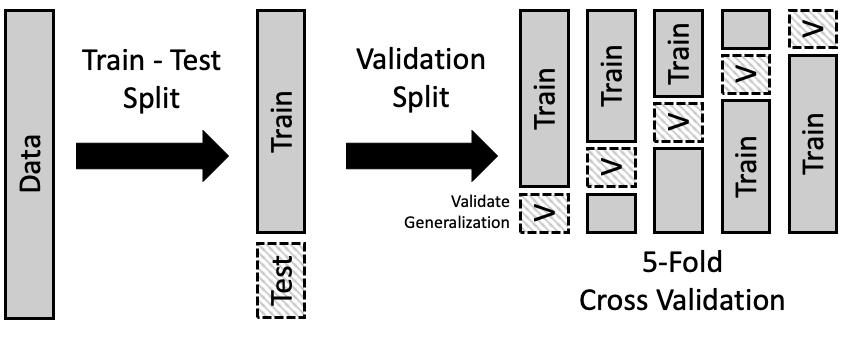
\includegraphics[width=0.95\textwidth]{capitulos/cap_02/imagenes/CVDiagram.png}
    \caption{
        Diagrama de división del dataset para la validación cruzada. 
        Recuperado de \cite{lau2023crossvalidation}.
    } 
    \label{fig:CVDiagram}
\end{figure}


% ------------------------------------------------------------------------------------------------------------
% ENSEMBLE LEARNING ------------------------------------------------------------------------------------------
% ------------------------------------------------------------------------------------------------------------

% \section{Ensemble Learning}

% El \textbf{aprendizaje por conjuntos (\textit{ensemble learning})} es una familia de técnicas de ML que 
% combina múltiples modelos de aprendizaje automático ---denominados \textbf{modelos base}--- para obtener un 
% modelo final con un mejor desempeño que los modelos base por separado.

% \subsection{Bagging}


% \subsection{Boosting}


% \subsection{Stacking}


% ------------------------------------------------------------------------------------------------------------
% DEEP LEARNING ----------------------------------------------------------------------------------------------
% ------------------------------------------------------------------------------------------------------------

\section{Deep Learning}

El \textbf{aprendizaje profundo (\textit{deep learning}, DL)} es una familia de técnicas de ML que utilizan 
múltiples capas de procesamiento para aprender representaciones de datos con varios niveles de abstracción
\cite{lecun2015}. Las redes neuronales han demostrado ser especialmente eficaces para este propósito, al 
permitir la composición jerárquica de características que capturan patrones cada vez más complejos en los 
datos.

Las redes neuronales tienen su origen en el intento de modelar las redes de neuronas del cerebro humano 
\cite{mcculloch1943}. Se requirió de numerosas contribuciones teóricas ---como el perceptrón 
\cite{rosenblatt1958} o el algoritmo de \textit{backpropagation} \cite{rumelhart1986,werbos1994}, entre 
otras---, disponibilidad de datos estandarizados y un gran aumento en la capacidad computacional para poder 
escalar estar redes y obtener resultados 
sorprendentes en tareas complejas.

Las \textbf{redes neuronales profundas (\textit{deep neural networks}, DNNs)} destacan por su capacidad para 
aprender representaciones jerárquicas: cada capa extrae características progresivamente más abstractas 
\cite{lecun2015}, desde líneas en imágenes hasta formas geométricas complejas, objetos completos e incluso 
escenas compuestas.
Esta propiedad las hace excepcionalmente versátiles, ya que procesan datos de muy diversa naturaleza ---datos 
tabulares, imágenes, audio, texto o señales temporales---, dados que ellas mismas aprenden los procesos de 
extracción de características de estos, hasta ahora realizados ``a mano'' (mediante procesos diseñados por la 
ingeniería de características) \cite{rusell2021} 
\footnote{
    Este enfoque se denomina aprendizaje extremo a extremo (\textit{end-to-end learning}), en el cual tanto la 
    extracción de características como la clasificación son parte de un modelo integral que se entrena de 
    manera conjunta, optimizando todos los componentes del sistema en un mismo proceso \cite{rusell2021}.
}. 
Gracias a ello, las DNNs han alcanzado rendimientos sobresalientes en dominios como visión por computador 
(clasificación de imágenes, detección de objetos, segmentación) o procesamiento de lenguaje natural 
(traducción, generación de texto) \cite{redhat2024DeepLearningDefinition}.
No obstante, su eficacia depende críticamente de grandes volúmenes de datos y recursos computacionales, lo que 
ha impulsado técnicas como el \textit{transfer learning} y modelos eficientes para democratizar su uso.


\subsection{El perceptrón multicapa}

El \textbf{perceptrón multicapa (\textit{multilayer perceptron}, MLP)} forma la base del \textit{deep 
learning}. Su diseño ---con capas ocultas, funciones de activación no lineales y entrenamiento  mediante 
\textit{backpropagation}--- sentó las bases conceptuales para arquitecturas más complejas, como las redes 
neuronales convolucionales o los \textit{transformers} \cite{murphy2022}. El MLP sigue siendo un referente 
teórico y la expresión más simple de cómo el aprendizaje jerárquico puede capturar patrones en los datos. 

Cada nodo en la red es denominado \textbf{unidad o neurona artifical}. Siguiendo el diseño propuesto en 
\cite{mcculloch1943,rosenblatt1958}, cada unidad recibe señales de entrada ---que o bien son las 
características de los datos o bien las salidas de las unidades de la anterior capa---, realiza una suma 
ponderada de estas con los pesos entrenables de cada conexión ---más un término independiente o sesgo, también 
entrenable---, aplica una función no lineal sobre esta para producir una salida que propaga a las unidades de 
la siguiente capa (véase la Figura \ref{fig:neuron_MLP}).

Matemáticamente, la operación de una unidad artifical se expresaría como:

$$
y = f \left( \sum_{i=1}^n{w_ix_i+b} \right)
$$

donde $x_i$ son las entradas, $w_i$ son los pesos entrenables ($w_0$ el sesgo)
\footnote{
    El sesgo se considera un peso, puesto que, en la implementación, son un peso más conectado a una unidad
    de sesgo con valor constante unitario (1).
}
, y $f$ es la función de activación.

\begin{figure}[h]
    \centering
    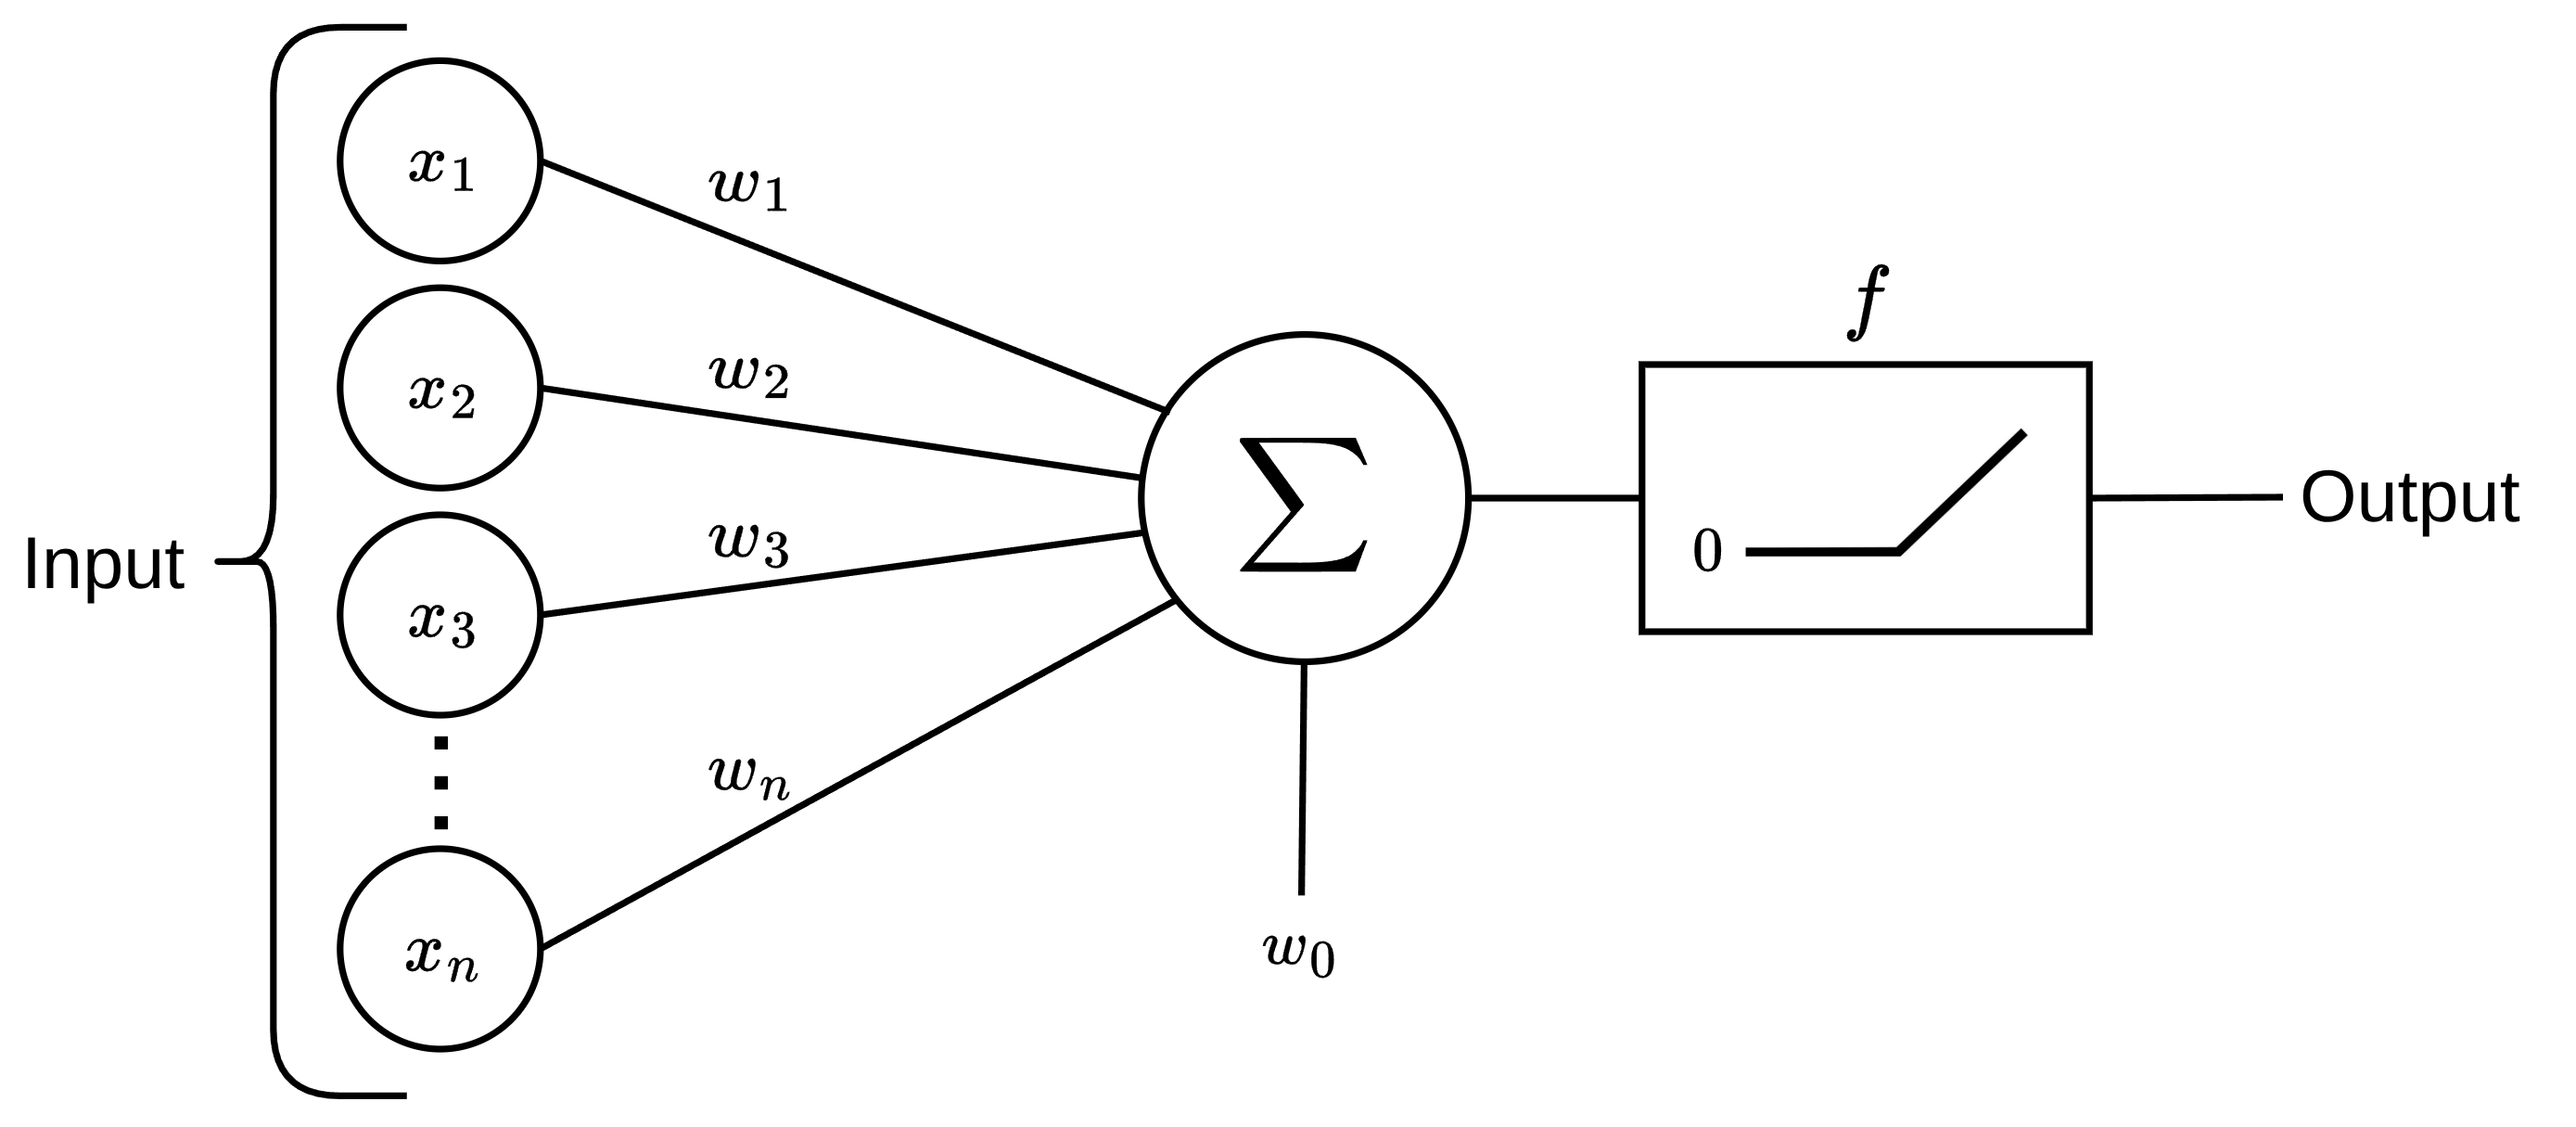
\includegraphics[width=0.95\textwidth]{capitulos/cap_02/imagenes/Neuron_perceptron.png}
    \caption{
        Esquema visual del funcionamiento de una unidad artificial. Adaptado de 
        \cite{codeworld2022understandingMLDL}.
    } 
    \label{fig:neuron_MLP}
\end{figure}


Esta \textbf{función de activación} a la salida de la unidad es un componente esencial que introduce no 
linealidad en el modelo, permitiendo a la red aprender relaciones complejas en los datos
\footnote{
    Sin ella, el MLP se reduciría a una simple combinación lineal de las entradas, incapaz de
    representar jerarquías de características \cite{murphy2022}.
}.
Existe multitud de funciones de activación, como la sigmoide, la tangente hiperbólica o ReLu ---y sus 
múltiples variantes---, cada una con sus ventajas y limitaciones
\footnote{
    Si bien, actualmente, ReLU y sus variantes (\textit{Leaky} ReLU, \textit{Parametric ReLU} o 
    \textit{Swish}) se han convertido en el estándar \textit{de facto} para las capas ocultas en DNNs,
    por su eficiencia computacional, y su eficacia empírica \cite{vargas2021}.
}.

La arquitectura de un MLP conecta estas unidades formando una red neuronal retroalimentada
\footnote{
    Una red neuronal retroalimentada (\textit{feed-forward neural network}) es aquella en la que las 
    conexiones entre las unidades no forman un ciclo y, por tanto, la información solo se mueve en una 
    dirección: adelante.
},
que consta de tres partes (véase la Figura \ref{fig:neural_network}):

\begin{itemize}

    \item \textbf{Capa de entrada}, en las que el número de unidades debe coincidir con el formato de entrada 
    de los datos, por ejemplo: en un problema con datos tabulares, debería haber una unidad por cada 
    característica.
    
    \item \textbf{Capas ocultas}, donde se realizan las transformaciones no lineales de los datos. Es en estas 
    donde el diseño puede variar en número de unidades y tipo de capas según la complejidad del problema y los 
    datos.
    
    \item \textbf{Capa de salida}, que proporciona el resultado del modelo. Su forma depende del problema a 
    resolver: 
    
    \begin{itemize}
        
        \item en problemas de regresión, esta capa tendrá tantas unidades como variables a predecir ---sin 
        función de activación, ya que esto limitaría el rango de valores posibles---;
        
        \item en problemas de clasificación, esta capa tendrá una sola unidad ---generalmente, con activación 
        sigmoide--- en clasificación binaria, o múltiples unidades ---con activación 
        \textit{softmax}
        \footnote{
            La activación \textit{softmax} no se aplica sobre la salida de una única unidad, sino que se 
            aplica sobre un vector de salidas de múltiples unidades, transformándolas en una distribución de 
            probabilidad, donde cada valor representa la probabilidad de pertenecer a una clase distinta y la 
            suma de todas las salidas es igual a 1.
        }
        --- en clasificación multiclase (véase la Figura \ref{fig:activation_func_classification}).
    \end{itemize}

\end{itemize}

\begin{figure}[h]
    \centering
    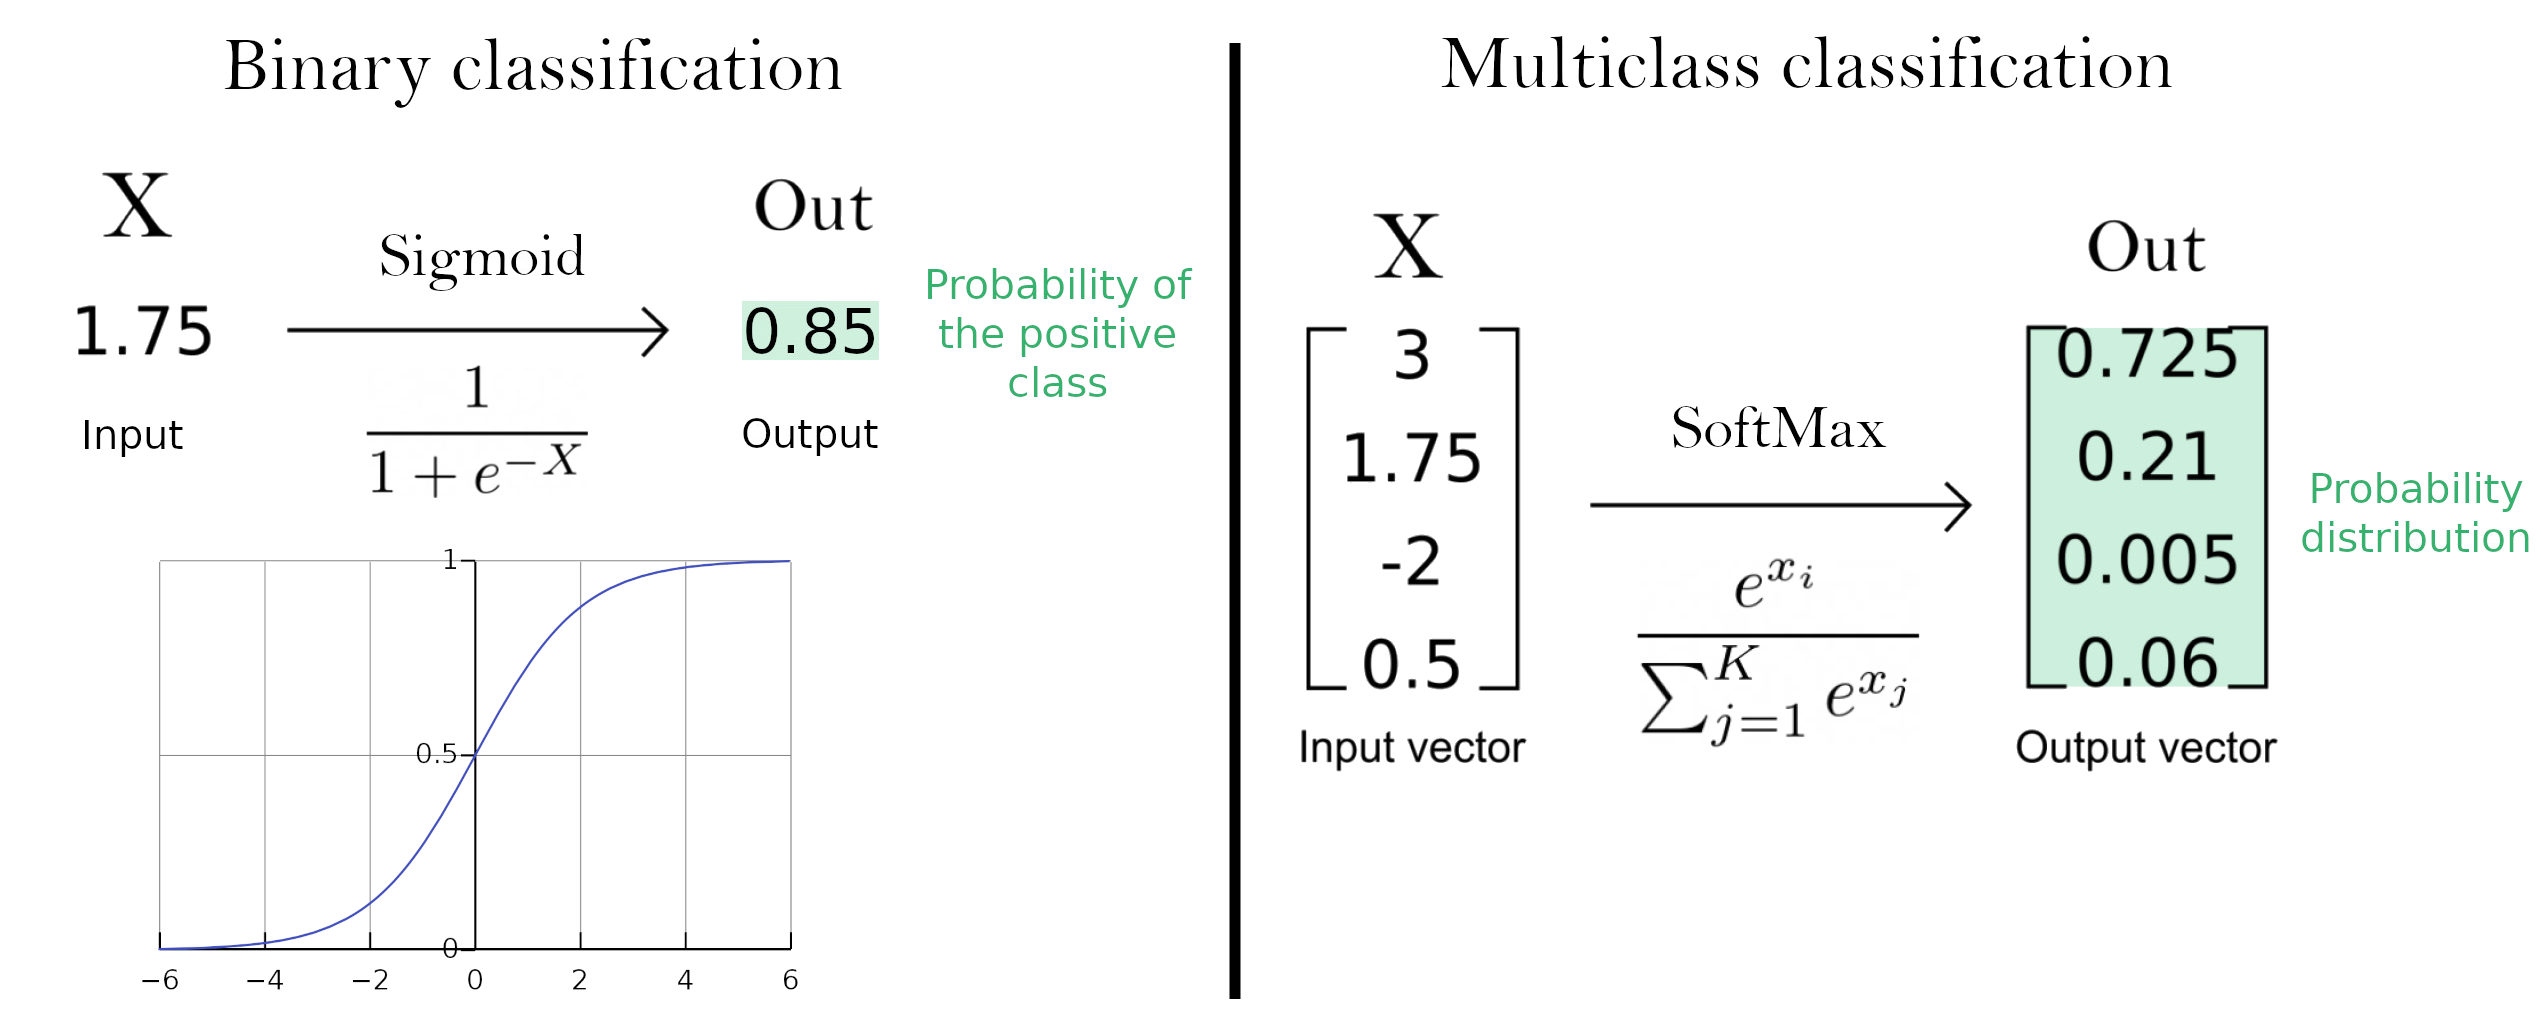
\includegraphics[width=\textwidth]{capitulos/cap_02/imagenes/ActivationFuncClassification.png}
    \caption{
        Diagrama de obtención de probabilidad en problemas de clasificación. 
        Adaptado de \cite{furnieles2022sigmoidandsoftmax}.
    } 
    \label{fig:activation_func_classification}
\end{figure}

%Quitar X y Out, y subir lo de abajo

\begin{figure}[h]
    \centering
    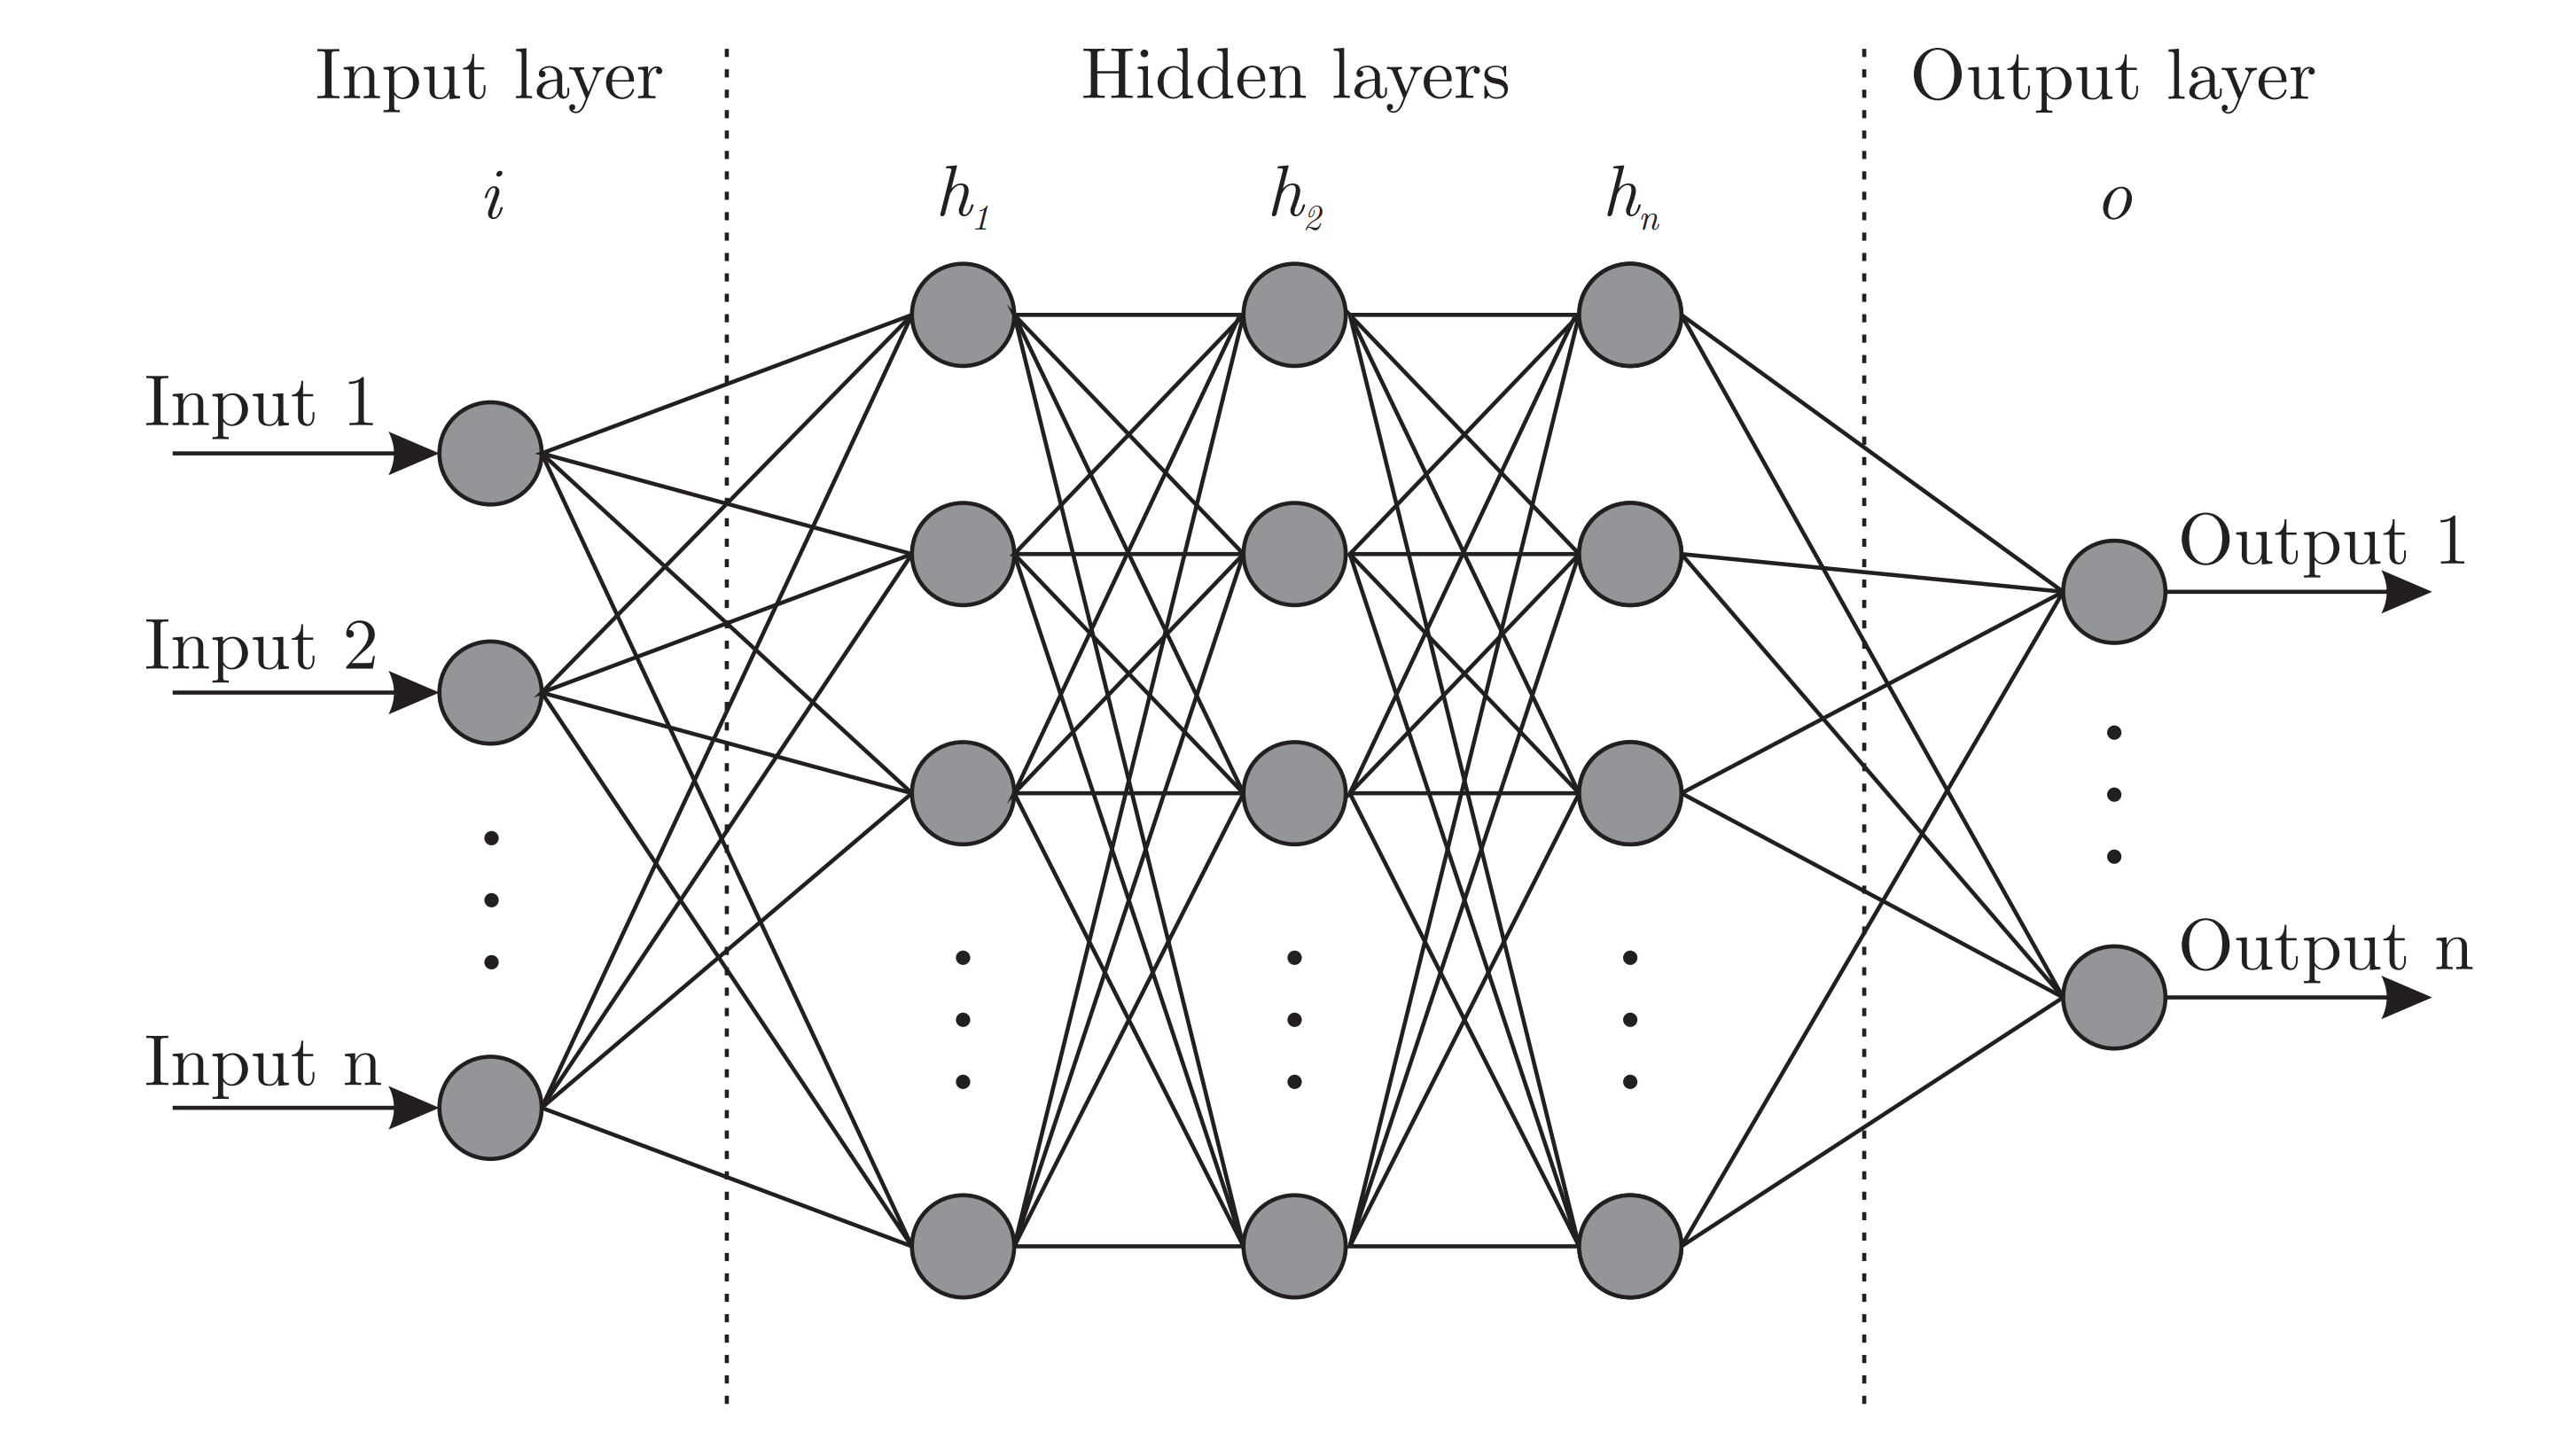
\includegraphics[width=0.95\textwidth]{capitulos/cap_02/imagenes/neural_network.png}
    \caption{
        Arquitectura simplificada de un MLP. 
        Recuperado de \cite{bre2017}.
    } 
    \label{fig:neural_network}
\end{figure}

% ------------------------------------------------------------------------------------------------------------

\subsection{Entrenamiento y validación de la red}

En el caso de las redes neuronales, el conjunto de datos suele dividirse en tres 
subconjuntos: entrenamiento, validación y prueba. A diferencia de métodos más tradicionales, no se utiliza 
validación cruzada, ya que entrenar redes profundas conlleva un elevado coste computacional.

Una vez hemos definido la arquitectura a emplear para resolver un problema, y definido los datos disponibles 
debemos entrenar la red con los datos de ejemplo. Este proceso implica ajustar los pesos del modelo para 
minimizar el error en las predicciones. 

El método de entrenamiento estándar en redes neuronales es el \textbf{algoritmo de retropropagación 
(\textit{backpropagation})}, que funciona en dos fases clave \cite{szeliski2010}:

\begin{itemize}

    \item \textbf{Propagación hacia adelante (\textit{forward pass})}: Los datos de entrada se procesan a 
    través de las capas de la red, generando una predicción. 

    \item \textbf{Propagación del error hacia atrás (\textit{backward pass})}: El error entre la 
    predicción y el valor real se calcula y se propaga hacia atrás en la red, ajustando los pesos mediante el 
    descenso de gradiente.
    
    Sin entrar en demasiado detalle, esto consiste en calcular el gradiente de la función de pérdida con           % Esto de "sin entrar en demasiado detalle" qué tal? 
    respecto a cada peso de la red, indicando cómo cada parámetro contribuye al error total. 
    A mayor aporte al error de un peso, más se ajustará ese peso. Así, el algoritmo priorizará modificar 
    significativamente los parámetros que más afectan al rendimiento de la red.
    
\end{itemize}

Este proceso explicado de manera vaga, tiene infinidad de detalles y variantes que influyen en su eficiencia y
eficacia:

\begin{itemize}

    \item El error obtenido entre la predicción y el valor real se calcula mediante la \textbf{función de 
    pérdida (\textit{loss function})}. Esta función cuantifica el error del modelo durante el entrenamiento, 
    midiendo la discrepancia entre las predicciones generadas y los valores o clases reales (\textit{ground 
    truth}).

    No se debe confundir con las métrica de evaluación de un modelo: aunque en algunos casos se pueden usar 
    métricas como funciones de pérdida y viceversa, las métricas destacan por ser fáciles de interpretar 
    y suele utilizarse más de una. En cambio, debe existir una únifa función de pérdida durante el 
    entrenamiento de una red neuronal, que debe cumplir tres requisitos clave:

    \begin{enumerate}

        \item Reflejar el objetivo del aprendizaje: Debe capturar adecuadamente qué significa ``éxito'' para 
        el modelo (p.ej., minimizar el error en regresión o maximizar la probabilidad de clasificación 
        correcta).

        \item Ser diferenciable: Es esencial para aplicar técnicas de descenso por gradiente, ya que el 
        optimizador necesita calcular derivadas.

        \item Ser eficiente computacionalmente: Dado que se evalúa en cada iteración del entrenamiento, su 
        cálculo debe ser rápido incluso con grandes volúmenes de datos.

    \end{enumerate}

    Mientras las métricas ayudan a entender el modelo, la función de pérdida es la que lo entrena.

    En problemas de regresión se emplean funciones de pérdida como el error cuadrático medio (\textit{mean 
    squared error}, MSE), que mide la diferencia promedio al cuadrado entre las predicciones y los valores 
    reales, o el error absoluto medio (\textit{mean absolute error}, MAE), que calcula la diferencia promedio 
    en valor absoluto
    \footnote{
        Aunque esta no es derivable en $x=0$, se define la derivada en ese punto como 0.
    }.

    En clasificación, las funciones de pérdida más comunes son la entropía cruzada (\textit{cross-entropy 
    loss}) para problemas de clasificación binaria y multiclase, que penaliza fuertemente las predicciones 
    incorrectas y ayuda a optimizar las probabilidades predichas para cada clase.


    \item Existen multitud de \textbf{algoritmos de optimización de parámetros}, como SGD, Adam o RMSProp. 
    Estos algoritmos determinan cómo actualizar los pesos del modelo durante el entrenamiento para minimizar 
    la función de pérdida. 
    Están basados en el descenso de gradiente, que ajusta los pesos en dirección opuesta al gradiente de 
    la función de pérdida respecto a los pesos, multiplicado por un factor escalar llamado \textbf{tasa 
    de aprendizaje (\textit{learning rate})}. Este hiperparámetro controla la magnitud de los pasos de 
    actualización: un valor demasiado alto puede hacer que el entrenamiento diverja, mientras que uno 
    demasiado bajo ralentiza la convergencia o estanca el modelo en mínimos locales.

    Existen estrategias avanzadas para ajustar el \textit{learning rate} de manera más eficiente durante el 
    entrenamiento, como la búsqueda de un \textit{learning rate} de punto de partida 


    \item Si bien existen métodos de entrenamiento de redes ejemplo a ejemplo ---como el Gradiente Descendente 
    Estocástico (SGD) puro\cite{bottou2010}---, estas se suelen entrenar por lotes 
    (\textit{minibatches})
    \footnote{
        Se denomina \textit{batch} al \textit{dataset} completo, y \textit{minibatch} a los subconjuntos de
        este cuyo tamaño está determinado por el hiperparámetro \textit{batch size}.
    } 
    debido a ventajas clave, como el aprovechamiento de la paralelización de operaciones en GPU y una mayor 
    estabilidad en la función de pérdida al promediarse el error entre varios ejemplos. 
    Aún así, establecer un tamaño de lote óptimo no es una tarea trivial que requiere de encontrar un 
    equilibrio entre generalización y velocidad: los lotes grandes aceleran el entrenamiento pero pueden 
    reducir la generalización del modelo, mientras que los lotes pequeños puede presentar una gran varianza 
    que introduzca ruido en el modelo \cite{keskar2017}, si bien esto puede ayudar a escapar de mínimos 
    locales, y puede paliarse con un bajo \textit{learning rate} (aunque esto aumentaría todavía más los 
    tiempos de entrenamiento).
    

    \item Tras el uso de \textit{minibatches} en el entrenamiento, surge el concepto de \textbf{época 
    (\textit{epoch})}, que hace referencia a un ciclo completo de presentación de todos los datos de 
    entrenamiento a la red neuronal \cite{rusell2021}. Durante una época, los \textit{minibatches} se procesan 
    secuencialmente, actualizando los pesos del modelo en cada iteración (o \textit{step}) con el gradiente 
    calculado sobre un lote. Por ejemplo, si un conjunto de entrenamiento tiene 4096 ejemplos y el tamaño de 
    lote es 32, una época constará de 128 iteraciones (4096/32).

    El número de épocas es un hiperparámetro crítico: demasiadas pueden llevar a sobreajuste 
    (\textit{overfitting}), donde el modelo memoriza los datos de entrenamiento pero no generaliza bien; 
    demasiado pocas pueden resultar en infraajuste (\textit{underfitting}), donde el modelo no captura los 
    patrones subyacentes. Además, la combinación de tamaño de lote y épocas influye en la dinámica de 
    optimización, ya que lotes más pequeños requieren más pasos por época, introduciendo más ruido pero 
    potencialmente mejorando la exploración del espacio de pesos.

    En la práctica, se suele establecer un número muy alto de épocas, y monitorizar el error en un conjunto de
    validación para determinar cuándo detener el entrenamiento, evitando así el sobreajuste cuando el error de
    validación comienza a aumentar. A esta técnica se le denomina \textbf{\textit{early stopping}} 
    \cite{goodfellow2016}.
    
\end{itemize}


% ------------------------------------------------------------------------------------------------------------

\subsection{Redes Neuronales Convolucionales}

Como ya se venía anticipando, la arquitectura MLP es especialmente adecuada para trabajar con datos 
estructurados o tabulares, donde la información se organiza en una matriz en la que cada columna representa 
una característica concreta (como sexo, altura o peso). 
Sin embargo, su diseño presenta limitaciones clave: al manejar vectores de entrada de tamaño fijo y carecer 
de mecanismos para aprovechar relaciones espaciales o secuenciales, no es óptima para datos no estructurados, 
como imágenes o texto, donde cada elemento individual (un píxel o una palabra) carece de significado por sí 
mismo \cite{murphy2022}.

Por ejemplo, los patrones aprendidos en una posición de una imagen podrían no ser reconocidos en otra 
ubicación, ya que las entradas tienen un recorrido distinto dentro de la red. Por tanto, el modelo carecería       % DUDA: Esto de que las entradas tienen un recorrido distinto en la red se entiende?
de \textbf{invarianza traslacional}, puesto que los pesos no se comparten entre distintas posiciones, a lo que 
se suma una marcada ineficiencia por el elevado número de parámetros requeridos \cite{szeliski2010}.

Precisamente para estos casos, otras arquitecturas profundas resultan más apropiadas.
Las \textbf{redes neuronales convolucionales (\textit{Convolutional Neural Network} en inglés, CNNs)} son un 
tipo de DNN que, aprovechando las ventajas de las operaciones convolucionales, explotan los principios de 
localidad y correlación espacial. Esto les permite procesar imágenes (en 1D, 2D o 3D) de manera eficiente, 
interpretando patrones visuales jerárquicos que un MLP no podría capturar, y con significativamente menos 
parámetros.


\subsubsection{Capas convolucionales}

Como se ha introducido antes, el operador de \textbf{convolución} es la base de las CNNs. Este operador 
matemático aplica un \textbf{filtro} (también denominado \textit{kernel})
\footnote{
    Aunque, como veremos después, a la hora de hablar de capas convolucionales, no son lo mismo.
} 
a regiones locales de una imagen de entrada, realizando un producto punto
\footnote{
    El producto punto o producto escalar de dos vectores, se define como la suma de los productos componente a 
    componente. 
    $$
    \mathbf{u} \cdot \mathbf{v} = \mathbf{u}_1 \cdot \mathbf{v}_1 + \mathbf{u}_2 \cdot \mathbf{v}_2 + ... + 
    \mathbf{u}_n \cdot \mathbf{v}_n
    $$
} 
entre los valores del filtro y los píxeles correspondientes de la imagen, y sustituyendo el valor del pixel 
central por el resultado del producto (véase la Figura \ref{fig:conv_op}).

\begin{figure}[h]
    \centering
    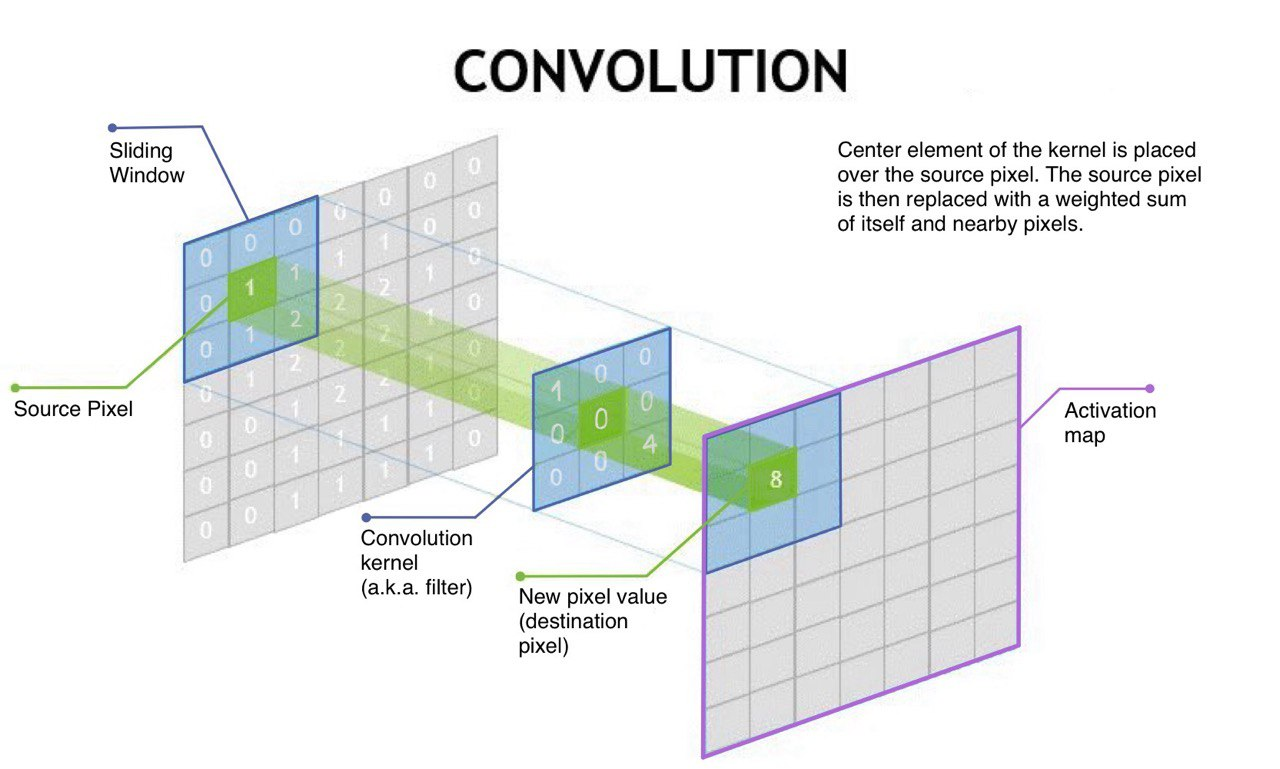
\includegraphics[width=0.95\textwidth]{capitulos/cap_02/imagenes/convolution_operation.jpg}
    \caption[Esquema gráfico de la aplicación de un filtro convolucional sobre una región de una imagen.]{
        Esquema gráfico de la aplicación de un filtro convolucional sobre una región de una imagen.
        Adaptado de \cite{nvidia2025convolutionoperation}.
    } 
    \label{fig:conv_op}
\end{figure}

Este proceso se repite al desplazar el filtro por toda la imagen mediante una \textbf{ventana deslizante}, 
generando un \textbf{mapa de activación}, que permite destacar líneas, curvas o texturas simples. Este mapa de
activación preserva la información de la localización de las características, si bien estas pueden ser 
detectadas en cualquier parte de la imagen. Esta propiedad se conoce como \textbf{equivarianza}. 

Las CNNs aprovechan la convolución mediante \textbf{capas convolucionales}. Cada capa convolucional está
compuesta por un conjunto de filtros convolucionales, donde cada uno a su vez tiene tantos \textit{kernels} 
como canales de entrada de la imagen haya en la capa (si es la primera capa convolucional, habrá 1 canal en 
imágenes de escala de grises, o 3 en imágenes RGB). El número de filtros en cada capa, su tamaño y la forma
en que se deslizan sobre la entrada
\footnote{                                                                      
    Definidos mediante los parámetros de \textit{stride} y \textit{padding}, que controlan el desplazamiento       
    del filtro y la cantidad de relleno alrededor de la entrada, respectivamente.
}
\todo{
    Añadir una imagen explicando stride y padding 
}
se determinan durante el diseño de la red, mientras que los valores de los \textit{kernels} son parámetros 
entrenables.

Cada filtro convolucional realiza la operación convolucional sobre cada canal con el \textit{kernel} que le 
corresponde. Después, se suman los mapas de activación de cada canal (pixel a pixel) añadiendo un sesgo 
(un mismo valor a todos los píxeles
\footnote{
    Es por ello que no rompe la propiedad de equivarianza.
}),
generando lo que denominamos como \textbf{mapa de características} (ya que idealmente extrae 
características relevantes). Los mapas de características generados con cada uno de los filtros son los nuevos 
canales, que conforman la salida de la capa convolucional. Esta salida puede ser posteriormente procesada por 
otras capas, permitiendo a la red aprender representaciones jerárquicas cada vez más abstractas de los datos 
de entrada: las primeras capas convolucionales detectarán bordes, cambios de color o texturas básicas; a 
medida que avanzamos en las capas de la red, las combinaciones de estas características simples permite 
identificar formas más complejas, como objetos e incluso composiciones.

Sin embargo, hemos pasado por alto algo fundamental: ¿cómo reunimos la información de dos regiones distantes 
de una imagen en un mismo sitio? Una primera aproximación intuitiva nos diría que los filtros convolucionales 
deben ser progresivamente más grandes, para capturar patrones de mayor tamaño y contexto. No obstante, esto
incrementaría considerablemente el número de parámetros y, por tanto, aumentaría el coste computacional y 
aumentaría el riesgo de sobreajuste del modelo (ya que un modelo con más parámetros puede memorizar mejor los
datos de entrenamiento). Es por esto que, en aquellos problemas en los que no es necesario preservar la 
información de localización de las características, ---como en los que nos enfocamos en este trabajo: 
clasificación y regresión---, y, por tanto, el modelo sea invariante a la ubicación, se emplean técnicas de 
submuestreo (\textit{downsampling}) \cite{murphy2022}, como usar \textit{stride} mayor de 1 en los filtros
de las capas convolucionales o realizar \textit{pooling}
\footnote{
    Nos centraremos en el último dado su amplio uso y fácil comprensión, además de su demostrada efectividad 
    empírica.
}.



\subsubsection{Capas de pooling}

Las \textbf{capas de agrupación (\textit{pooling layers})} tienen como objetivo principal comprimir la 
información de la imagen, reduciendo sus dimensiones (alto y ancho) mientras se preservan los datos más 
relevantes para la tarea. Esta reducción del tamaño espacial de los mapas de características disminuye el 
número de parámetros y operaciones en las fases posteriores, lo que reduce el coste computacional. Además, 
tiene un beneficio adicional: ayuda a prevenir el sobreajuste, ya que al limitar la cantidad de parámetros, 
el modelo evita memorizar ruido o detalles irrelevantes de los datos de entrenamiento, favoreciendo así el 
aprendizaje de patrones generalizables.

Hay diversos métodos de \textit{pooling}, entre los que destacan:

\begin{itemize}

    \item \textbf{Max pooling}, que calcula el máximo valor de regiones del mapa de características, y lo
    usa para crear un mapa de características reducido (véase la Figura \ref{fig:max_pooling}).

    \item \textbf{Average pooling}, que reemplaza el valor máximo del \textit{max pooling} por el cálculo de
    la media entre los valores de la región. 

\end{itemize}

La región de aplicación del \textit{pooling}, al igual que en la convolución, viene determinada por ciertos 
parámetros, definidos por el diseñador, como el tamaño de filtro (que suele ser de 2x2), el \textit{stride} 
y el \textit{padding}, si bien también existen variantes  adaptativas (\textit{adaptive}), que ajustan
automáticamente su cobertura para producir una salida con dimensiones específicas, independientemente del 
tamaño de la imagen de entrada. Esta funcionalidad es especialmente útil cuando se necesita adaptar los mapas
de características para conectarlos a una capa \textit{fully-connected}. 

\begin{figure}[h]
    \centering
    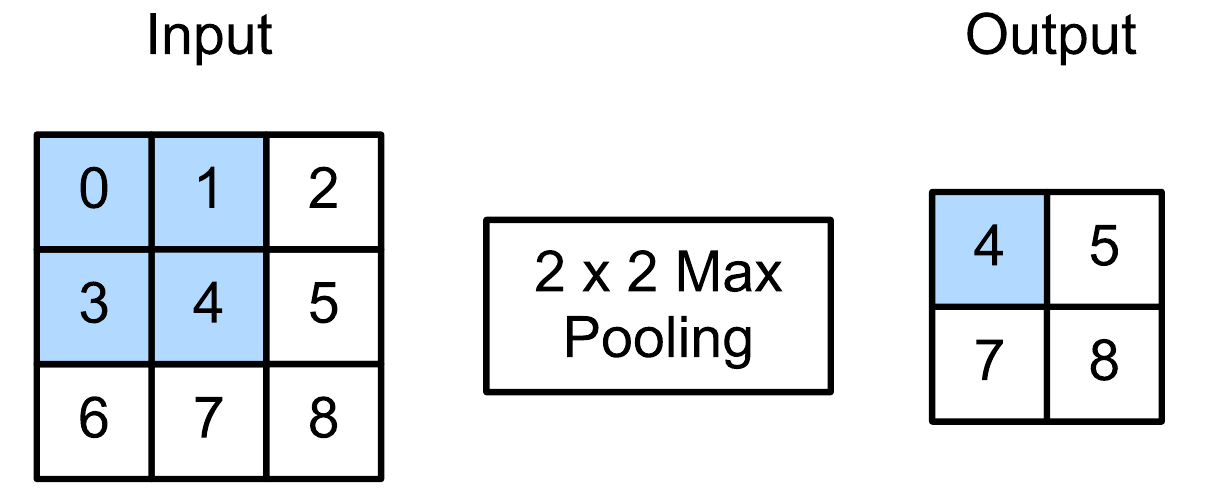
\includegraphics[width=0.7\textwidth]{capitulos/cap_02/imagenes/max_pooling.png}
    \caption{
        Esquema gráfico de \textit{max pooling} con un filtro 2x2 y \textit{stride} de 1.
        Recuperado de la Figura 14.12 de \cite{murphy2022}.
    } 
    \label{fig:max_pooling}
\end{figure}



\subsubsection{Capas \textit{Fully-Connected}}

Como hemos visto hasta ahora, en las CNNs, las primeras capas están diseñadas para extraer características
espaciales a través de filtros convolucionales y de \textit{pooling}. Sin embargo, una vez que se ha reducido 
la dimensionalidad y se han obtenido representaciones abstractas de alto nivel, es necesario realizar una 
predicción (en problemas de clasificación y regresión). 
Aquí es donde las \textbf{capas completamente conectadas (\textit{fully-connected}, FC)} juegan un papel 
crucial. Se utilizan en las últimas etapas de la red convolucional para combinar todas las características 
extraídas y producir una predicción final. Es decir, actúan como el clasificador/regresor
\footnote{
    Si bien, independientemente de la tarea ---regresión o clasificación---, a esta parte de la red se le 
    denomina clasificador
} 
que toma todas las señales procesadas por las capas anteriores y predice la clase a la que pertenece la imagen 
o el valor objetivo. 

La arquitectura de esta capa sigue la estructura del MLP, con neuronas organizadas en una o más capas densas, 
donde cada neurona está conectada con todas las salidas de la capa anterior. Para que esto sea posible, 
primero se aplica una operación de \textbf{\textit{flattening}} que transforma el mapa de características 
multidimensional en un vector unidimensional. A partir de ahí, el procesamiento es equivalente al de una red 
neuronal tradicional: cada neurona calcula una combinación lineal de sus entradas seguida de una función de 
activación no lineal.


\subsubsection{Diseño de la CNN para problemas de clasificación y regresión}

Un patrón común de diseño de CNNs para la resolución de problemas de clasificación y regresión consta de dos
componentes principales:

\begin{itemize}

    \item el \textit{backbone} o extractor de características, que alterna capas convolucionales con capas de
    \textit{pooling}, cuya función es extraer representaciones jerárquicas y cada vez más abstractas de los 
    datos de entrada; y

    \item el \textit{classifier}, generalmente implementado mediante una o más capas totalmente conectadas, 
    toma estas representaciones para realizar la tarea específica de salida, ya sea clasificación o regresión.

\end{itemize}


\begin{figure}[h]
    \centering
    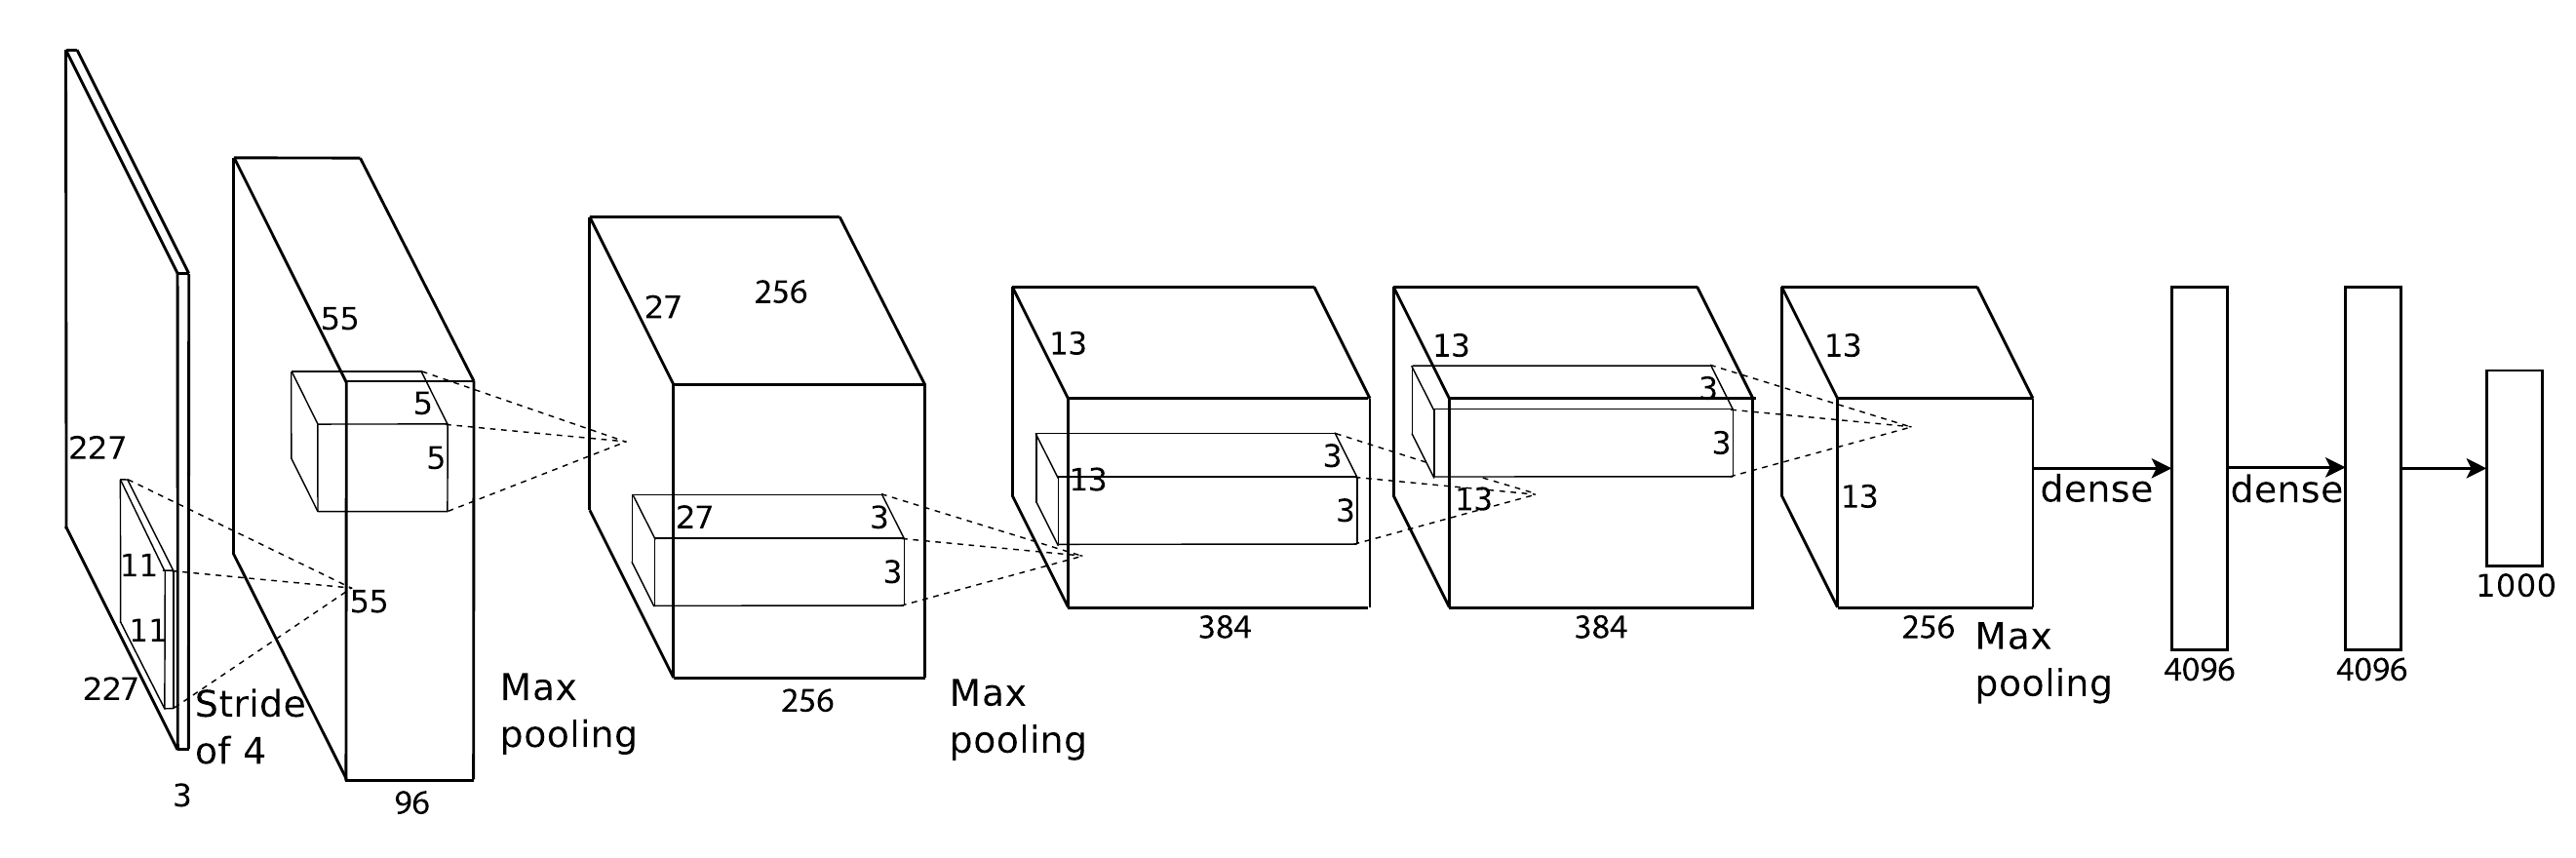
\includegraphics[width=0.95\textwidth]{capitulos/cap_02/imagenes/CNN_complete.png}
    \caption[
        Esquema gráfico de la arquitectura conocida como ``AlexNet'', diseñada para resolver un problema
        de clasificación con 1000 clases.
        Recuperado de la Figura 5.39 de \cite{szeliski2010}.
    ]{
        Esquema gráfico de la arquitectura conocida como ``AlexNet'', diseñada para resolver un problema
        de clasificación con 1000 clases.
        Recuperado de la Figura 5.39 de \cite{szeliski2010}.
        Esta arquitectura presenta una serie de capas convolucionales con funciones de activación no lineales 
        ReLU, max pooling, algunas capas totalmente conectadas y una capa final \textit{softmax}, la cual se 
        alimenta a una función de pérdida de entropía cruzada multiclase.
    } 
    \label{fig:CNN_complete}
\end{figure}


\subsubsection{Regularización y normalización}

Como en otras arquitecturas de redes neuronales, existen numerosas técnicas de regularización para evitar
el sobreajuste. Veamos algunas de las técnicas empleadas en CNNs:

\begin{itemize}

    \item \textbf{\textit{Data augmentation}} \cite{chen2019,zhang2021}: Consiste en añadir o modificar 
    dinámicamente ejemplos a partir de los que se tienen originalmente, de forma que se entrene la red con 
    un conjunto de datos más diverso y robusto, evitando el sobreajuste y mejorando la generalización.
    
    Algunas alteraciones realizadas pueden ser cambios en el nivel de brillo y contraste, rotaciones, 
    traslaciones, escalados o volteos de imágenes, entre otras. No existe configuración óptima, y su 
    configuración depende mucho del problema y las imágenes disponibles.

    Esta técnica sirve especialmente para problemas como clasificación o regresión, donde las clases o valores 
    predichos no suelen variar bajo pequeñas perturbaciones locales. 
    
    \item \textbf{\textit{Dropout}} \cite{srivastava2014}: Técnica que, durante el entrenamiento, ``apaga'' 
    (pone a cero) aleatoriamente un porcentaje de neuronas en cada iteración, evitando así que la red 
    dependa demasiado de determinadas unidades individuales (véase la Figura \ref{fig:net_with_dropout}). 
    En CNNs suele aplicarse a capas \textit{fully-connected}, 
    aunque existen variantes como \textit{Spatial Dropout} \cite{tompson2015} que elimina canales completos 
    en capas convolucionales, forzando una distribución más robusta de características.

    \begin{figure}[h]
        \centering

        \begin{subfigure}[b]{0.45\textwidth}
            \centering
            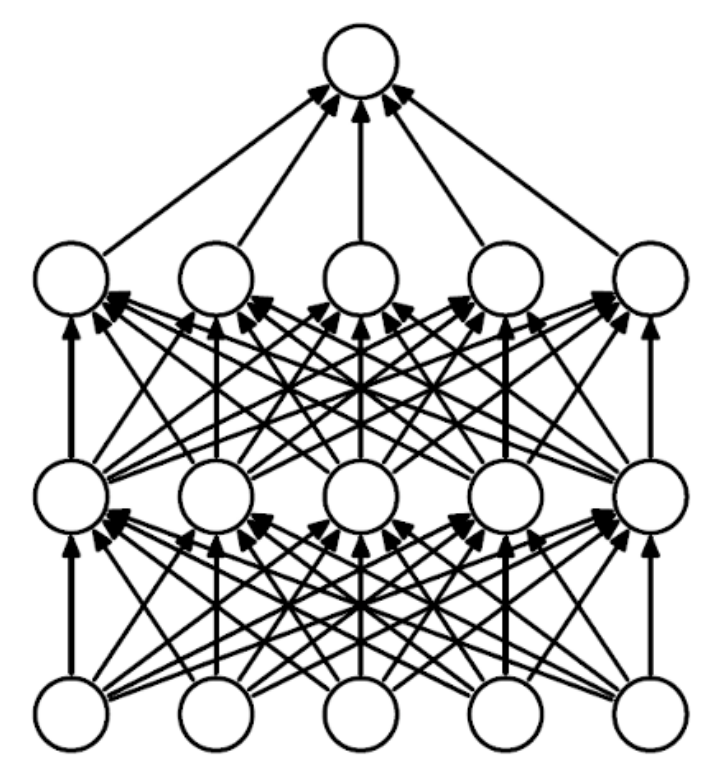
\includegraphics[width=\textwidth]{capitulos/cap_02/imagenes/net_without_dropout.png}
            \caption{Dropout desactivado}
            \label{fig:net_deactivate_dropout}
        \end{subfigure}
        \hfill
        \begin{subfigure}[b]{0.45\textwidth}
            \centering
            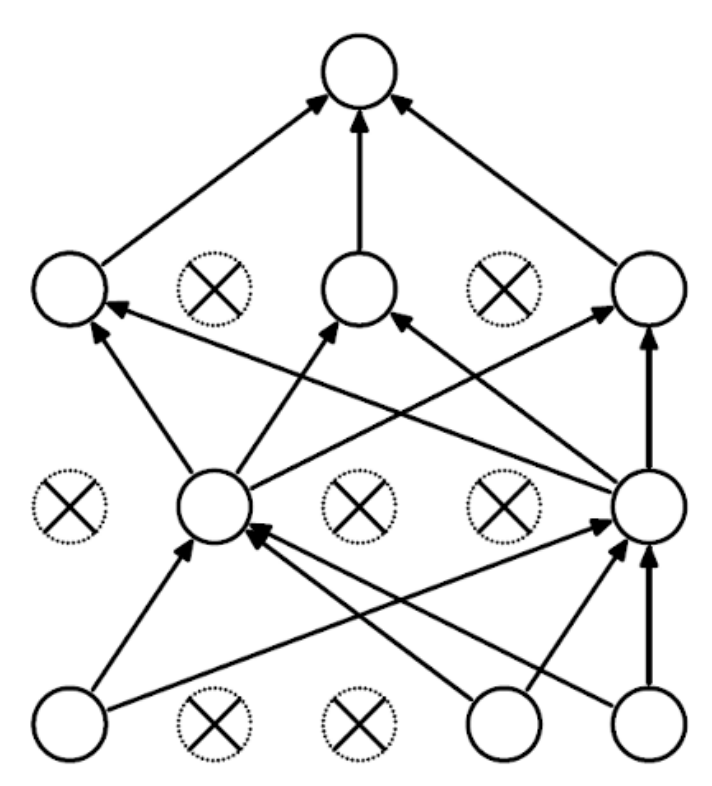
\includegraphics[width=\textwidth]{capitulos/cap_02/imagenes/net_with_dropout.png}
            \caption{Dropout activado ($p=0.5$)}
            \label{fig:net_activate_dropout}
        \end{subfigure}

        \caption[
            Diagrama del funcionamiento de neuronas con \textit{dropout}.
            Recuperado de la Figura 5.29 de \cite{szeliski2010}.
        ]{
            Diagrama del funcionamiento de neuronas con \textit{dropout}.
            Recuperado de la Figura 5.29 de \cite{szeliski2010}.
            Cuando se evalúa el modelo, todas las unidades funcionan correctamente 
            (\ref{sub@fig:net_deactivate_dropout}). Durante el entrenamiento, algunas son ``apagadas'' 
            (\ref{sub@fig:net_activate_dropout}). 
        }
        \label{fig:net_with_dropout}
    \end{figure}
    
    \item \textbf{\textit{Batch normalization}} \cite{ioffe2015}: Esta se introduce como una capa nueva a 
    añadir en el diseño de las redes, con nuevos parámetros entrenables: \textit{scale} y \textit{shift}. 
    Normaliza los valores de cada canal (media cero y desviación 1), y los reescala y desplaza en base a los
    valores de \textit{scale} y \textit{shift}. 
    Esto suaviza significativamente el espacio de valores de optimización \cite{santurkar2019} y reduce la 
    sensibilidad a la tasa de aprendizaje \cite{arora2018}, permitiendo establecer valores más altos.
    En CNNs se aplica típicamente después de las capas convolucionales y antes de la función de activación
    
\end{itemize}


\subsubsection{Conexiones residuales}

Uno de los principales problemas que no permite aumentar mucho la profundidasd de las redes convolucionales 
es el desvanecimiento de gradiente (\textit{vanishing gradient problem}), que consiste en la disminución 
exponencial de los gradientes durante el proceso de \textit{backpropagation} a medida que se retrocede hacia 
las capas iniciales de la red. Algunas de las soluciones a este problema han sido: utilizar funciones de 
activación ReLU, ya que evita gradientes pequeños para valores positivos; inicializar adecuadamente los pesos
de la red; o \textit{batch normalization}, que estabiliza la distribución de las activaciones. Sin embargo,
las conexiones residuales han sido la contribución más significativa para resolver este problema.

Las \textbf{redes residuales (\textit{residual nets}, ResNet)} 

%https://www.jeremyjordan.me/nn-learning-rate/



% ------------------------------------------------------------------------------------------------------------

\subsection{Transfer Learning}

El \textbf{aprendizaje por transferencia (\textit{transfer learning})} es una técnica que consiste en 
aprovechar el conocimiento aprendido por un modelo entrenado en una tarea como punto de partida para
mejorar el rendimiento y acelerar el entrenamiento en una nueva tarea relacionada \cite{rusell2021}.

En redes neuronales, el aprendizaje consiste en ajustar pesos, y en el caso del \textit{transfer learning}, 
estos pesos se inicializan con valores previamente optimizados para una tarea fuente, en lugar de comenzar con 
valores aleatorios (véase la Figura \ref{fig:fine-tuning}).

Se conoce como \textbf{fine-tuning} a la técnica de inicialización de los pesos de aquellas partes del modelo 
(como capas convolucionales) con los pesos previamente aprendidos, y que continúa el entrenamiento con los 
datos específicos de la nueva tarea. En este contexto, se denomina \textit{head} a las capas finales del 
modelo que se sustituyen para adaptarse a la nueva tarea. 

\begin{figure}[h]
    \centering
    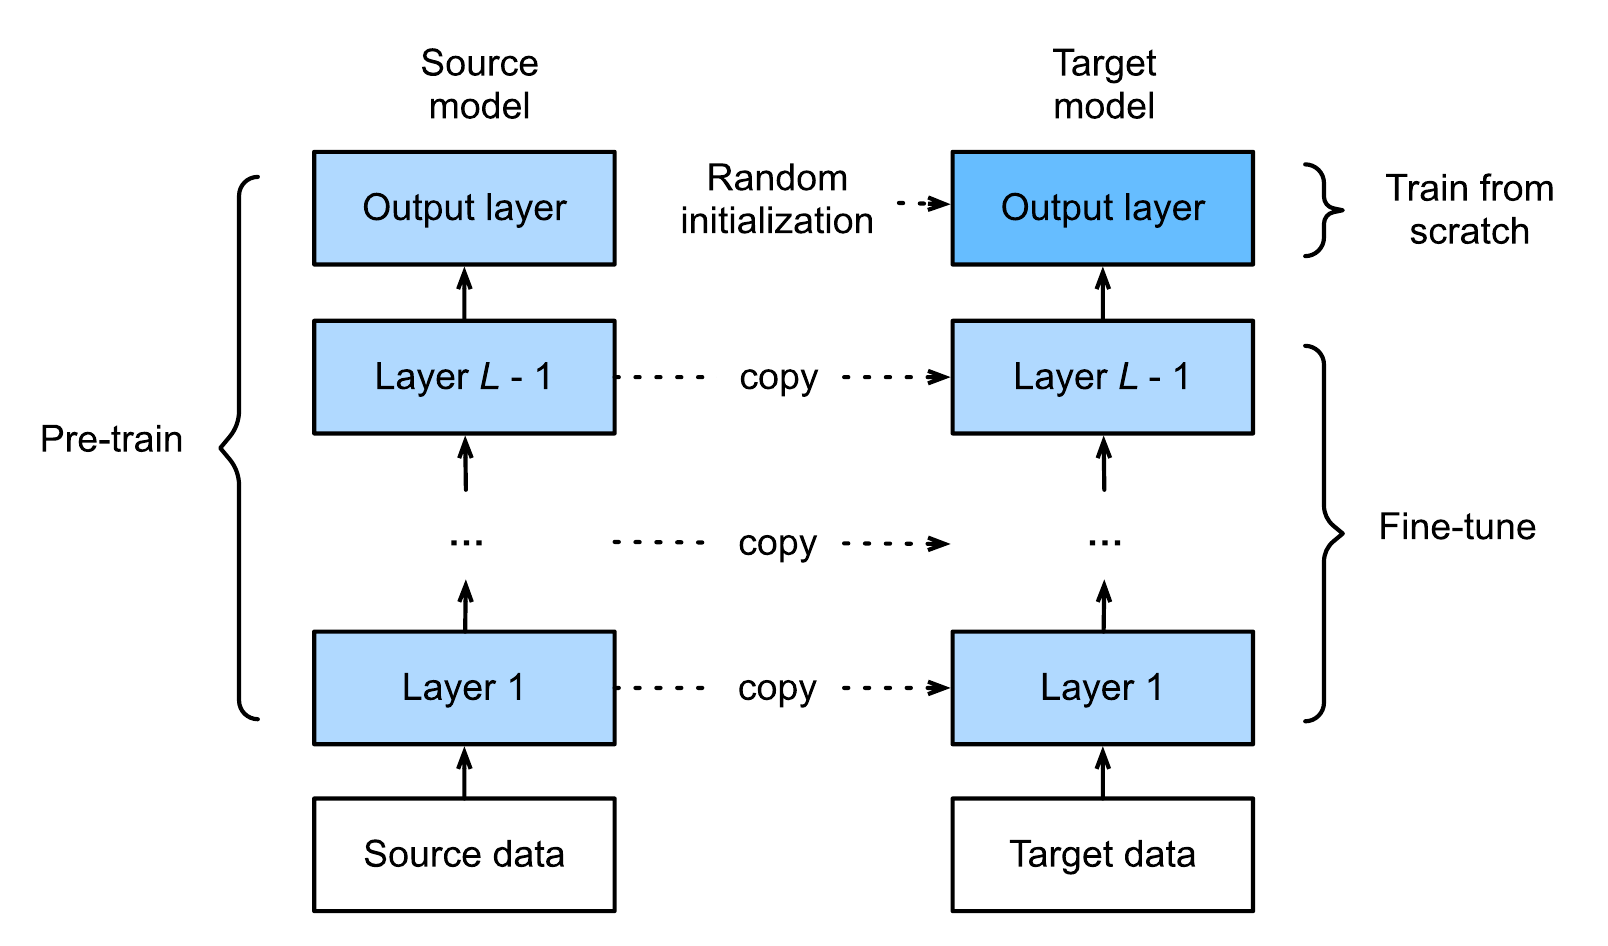
\includegraphics[width=0.95\textwidth]{capitulos/cap_02/imagenes/fine-tunning.png}
    \caption[
        Diagrama de \textit{fine-tuning} de un modelo en una nueva tarea. 
        Recuperado de la Figura 19.2 de \cite{murphy2022}.
    ]{
        Diagrama de \textit{fine-tuning} de un modelo en una nueva tarea. 
        Recuperado de la Figura 19.2 de \cite{murphy2022}.
        La capa final de salida es entrenada desde cero para la nueva tarea. El resto de capas son 
        inicializadas con los pesos previos. 
    } 
    \label{fig:fine-tuning}
\end{figure}

Por ejemplo, en \cite{venema2022} se utilizan dos modelos de CNN preentrenados en clasificación con ImageNet 
(que contiene imágenes de 1000 clases): VGG16 y ResNet50. Estos modelos se ajustan (\textit{fine-tuning}) 
para estimar el sexo de una persona a partir de radiografías de húmero. Aunque ambas tareas parecen muy 
diferentes, las primeras capas de la red, especializadas en detectar características generales como bordes y 
texturas, pueden ser útiles en los dos casos, lo que permite una transferencia efectiva del conocimiento.

El \textit{fine-tuning} puede aplicarse de forma gradual: primero se entrena solo el \textit{head} 
(manteniendo el resto del modelo congelado) y luego, si es necesario, se afinan también algunas capas 
preentrenadas para mejorar el rendimiento en la tarea específica.


% ------------------------------------------------------------------------------------------------------------
% INCERTIDUMBRE ----------------------------------------------------------------------------------------------
% ------------------------------------------------------------------------------------------------------------

\section{Incertidumbre}

La metrología
\footnote{
    Ciencia de las mediciones y sus aplicaciones \cite{jcgm200:2012}.
},
y la estadística comparten un papel fundamental en el análisis del error y la incertidumbre en campos como 
el ML. Mientras la metrología establece los fundamentos conceptuales de error e incertidumbre, la estadística 
proporciona métodos para cuantificar, modelar y reducir estos factores durante el desarrollo y validación de 
modelos.

El Comité Conjunto de Guías en Metrología (\textit{Joint Committe for Guides in Metrology})
\footnote{
    Este Comité está formado por numerosas organizaciones internacionales de metrología y normalización: 
    BIPM, IEC, IFCC, ISO, IUPAC, IUPAP, OIML e ILAC. Su objetivo principal es mantener y promover las 
    guías internacionales clave en metrología, como la Guía para la Expresión de la Incertidumbre en la 
    Medición (\textit{Guide to the Expression of Uncertainty in Measurement}, GUM) \cite{jcgm100:2008} y el 
    Vocabulario Internacional de Metrología (\textit{Vocabulaire international de métrologie}, VIM) 
    \cite{jcgm200:2012}.
}
define el \textbf{error} como una ``medición imperfecta'' de la magnitud observada, que puede estar causada
por efectos aleatorios (componente aleatoria del error) y por efectos sistemáticos (componente sistemática del 
error, más conocida como \textbf{sesgo}).
Por otro lado, define a la \textbf{incertidumbre} como ``parámetro, asociado con el resultado de una medición, 
que caracteriza la dispersión de los valores que podrían atribuirse razonablemente al \textbf{mensurado}, que
es como se denomina a la magnitud a ser medida. [...] El parámetro puede ser, por ejemplo, una desviación 
estándar, o la anchura de un intervalo con un nivel de confianza establecido'' \cite{jcgm100:2008}.

Partiendo de estas definiciones generales, veamos las diferencias entre los dos enfoques principales en la 
evaluación de mediciones: el enfoque basado en el error y el enfoque basado en la incertidumbre.

El \textbf{enfoque basado en el error} o enfoque tradicional parte de la premisa de que existe un valor 
verdadero. En consecuencia, el propósito de la medición es aproximarse lo más posible a dicho valor, 
minimizando las distintas componentes del error \cite{jcgm100:2008}:

\begin{itemize}
    \item para el error aleatorio, esto se logra aumentando el número de observaciones, ya que su distribución 
    tiene una media igual a cero; y

    \item para el error sistemático, es necesario identificarlo y cuantificar su magnitud, lo que permite 
    aplicar factores de corrección que compensen su efecto.

\end{itemize}

Se asume que el resultado de la medición ha sido corregido por todos los efectos sistemáticos identificados
como significativos, de modelo que la esperanza matemática de esta componente sea igual a cero.

Sin embargo, en la práctica no existen reglas claras para distinguir las componentes del error ni cómo estas 
se combinan en el error total
 que permitan diferenciar claramente las componentes del error ni
cómo estas se combinan en el error total. En general, solo es posible estimar un límite superior del valor 
absoluto del error total estimado, al que se denomina de forma inapropiada ``incertidumbre''. 

Frente a enfoque anterior, se presenta el \textbf{enfoque basado en la incertidumbre} \cite{jcgm100:2008}, 
cuyo propósito no es hallar el mejor valor posible, sino establecer un intervalo de valores razonables para el 
mensurando, el cual puede refinarse con información adicional. Así, la medición misma se convierte en una 
herramienta para determinar el error del instrumento. 

% ------------------------------------------------------------------------------------------------------------

\subsection{Intervalos de valores razonables}

\todo{Creo que es mejor eliminar este apartado e incluirlo en el anexo pero lo dejo por ahora para 
que vea la diferencia entre el intervalo de confianza, el de credibilidad y el de predicción}

Veamos qué tipos de intervalos de valores nos permiten cuantificar la variabilidad de los resultados y, por 
tanto, la incertidumbre de la medición realizada. 

\begin{itemize}

    \item El \textbf{intervalo de confianza (IC)} es una herramienta común de la estadística 
    frecuentista
    \footnote{
        La estadística frecuentista ... ¿Anexo explicando las diferencias entre frecuentista y bayesiana?
        (para agosto)
    },
    que permite estimar un rango de valores tal que podamos confiar en que contiene al valor verdadero de 
    un parámetro poblacional desconocido $\theta$ (p.ej., la media) \cite{berrendero2025}.

    Los métodos del cálculo del IC dependen de la distribución del estimador (p.ej., la distribución de la
    media muestral) y los parámetros conocidos. 

    Es importante aclarar un malentendido común: un intervalo de confianza con nivel 95\% para un parámetro 
    $\theta$ no significa que exista un 95\% de probabilidad de que $\theta$ esté dentro del intervalo 
    calculado a partir de una muestra específica. En realidad, el 95\% se refiere a la frecuencia con la que 
    , si muestreásemos muchas veces los datos, los intervalos construidos a partir de esas muestras incluirían 
    al valor verdadero de $\theta$ en aproximadamente el 95\% \cite{murphy2022}.


    \item El \textbf{intervalo de credibilidad o región creíble (RC)} es, de hecho, la que determina que el 
    parámetro $\theta$ está contenido en el rango de sus valores con una probabilidad determinada por la 
    confianza. Este intervalo es la aproximación bayesiana equivalente al intervalo de confianza, y, como 
    este, requiere conocer la distribución a priori de los datos.

    La diferencia radica en que, a diferencia del intervalo de confianza, que parte de que $\theta$ es un 
    parámetro fijo desconocido y los datos son tratados como aleatorios, el enfoque bayesiano fija los datos
    (ya que son conocidos) y el parámetro $\theta$ lo trata como aleatorio (ya que es desconocido) 
    \cite{murphy2022}.

    Esta interpretación resulta más intuitiva y directa en comparación con la interpretación frecuentista del 
    intervalo de confianza. En particular, una región creíble del 95\% sí puede interpretarse como que hay un
    95\% de probabilidad de que el parámetro $\theta$ se encuentre dentro de ese intervalo, dado el conjunto
    de datos observado y la distribución a priori asumida.

    \todo{Incluir imagen comparando intervalo de confianza y credibilidad}


    \item El \textbf{intervalo de predicción (\textit{prediction interval})} es radicalmente diferente a los 
    intervalos previos, pues trata de predecir un valor futuro de una observación, no determinar un parámetro 
    poblacional. Existen numerosos métodos, con mayores y menores garantías estadísticas, con y sin 
    necesidad de conocer la distribución de los datos. El enfoque más prometedor es la predicción conformal, 
    que han demostrado ser eficaz en contextos donde los supuestos clásicos (normalidad, homocedasticidad) no 
    se cumplen \cite{romano2019}, y es actualmente el enfoque más robusto para la construcción de intervalos 
    de predicción en aplicaciones modernas de ML 
    \cite{romano2019, luo2025, sadinle2019, romano2020, angelopoulos2020}.

\end{itemize}

% Relacionándolo con el apartado anterior, los intervalos de confianza solo informan de la incertidumbre 
% aleatoria, puesto que asumen que el modelo está bien especificado y que el error residual es la única fuente 
% de variabilidad. 

% Los intervalos de credibilidad sí integran la incertidumbre en los parámetros del modelo y en la estructura 
% del modelo mismo, capturando así tanto la incertidumbre aleatoria como la incertidumbre epistémica.

% Frente a estos, los intervalos de predicción obtenidos mediante predicción conformal sí presentan información
% de los tres componentes de incertidumbre. 

Como podemos esperar, a más estrecho sea el intervalo que manejemos, más se puede confiar en las predicciones,
pero no todos los tipos de intervalos revelan la misma información sobre incertidumbre. 

% ------------------------------------------------------------------------------------------------------------

\subsection{Incertidumbre en \textit{machine learning}}

El enfoque basado en incertidumbre se puede extrapolar a modelos de ML, incorporando técnicas de 
\textbf{cuantificación de la incertidumbre (\textit{Uncertainty Quantification}, UQ)} para evaluar y comunicar 
la confianza del modelo en sus predicciones. 
En problemas de regresión, la analogía es directa: es deseable que los modelos no solo proporcionen una 
predicción puntual, sino también un intervalo que indique el grado de incertidumbre asociado a cada 
predicción, conocido como \textbf{intervalo de predicción (\textit{prediction interval})},
el cual puede derivarse de métodos de UQ como \textit{bootstrapping} o predicción conformal
En caso de los problemas de clasificación, el concepto equivalente
al de intervalo de predicción se denomina \textbf{conjunto de predicción (\textit{prediction set})}, 
que puede construirse mediante técnicas como estimaciones de probabilidad calibrada o predicción conformal.  

Las fuentes de incertidumbre pueden ser muy variadas, y su identificación requiere en muchos casos de 
conocimiento específico en el problema. Si bien se suelen considerar dos tipos de incertidumbre en las 
predicciones realizadas en ML \cite{hullermeier2021}:

\begin{itemize}
    
    \item La \textbf{incertidumbre aleatoria} es la relativa al dato individual. 
    Esta incertidumbre se debe a la variabilidad inherente del fenómeno observado y no puede reducirse, aunque 
    se disponga de más datos. Por ejemplo, en un entorno médico, puede reflejar la variabilidad entre 
    pacientes con condiciones similares.

    \item La \textbf{incertidumbre epistémica} es la causada por falta de conocimiento o precisión del modelo.
    Se relaciona con aspectos como la escasez de datos, la calidad de la información disponible o la capacidad 
    limitada del modelo para generalizar. A diferencia de la incertidumbre aleatoria, la epistémica es 
    reducible: puede disminuirse con más datos, mejores modelos o mayor comprensión del problema.
    
\end{itemize}

A estos, se le puede añadir un tercero: el \textbf{\textit{drift}} \cite{gama2012}, que procede de cambios en 
la distribución de los datos a lo largo del tiempo, ya sea en la distribución de las variables de entrada, en 
la distribución de las variables de salida, o en la relación entre las dos previas. Por ejemplo: una imagen 
de entrada a un modelo de clasificación que no corresponde a ninguna clase con la que se haya entrenado 
anteriormente, un cambio en la población objetivo de una aplicación médica ---p.ej., debido a un cambio 
demográfico o a la aparición de una nueva enfermedad---, entre otros. 

% ------------------------------------------------------------------------------------------------------------

\subsection{Cuantificación de la incertidumbre en \textit{machine learning}}

La cuantificación de la incertidumbre puede abordarse desde dos perspectivas: 

\begin{itemize}
    
    \item sobre nuevos datos (no vistos), donde el objetivo es estimar la confianza del modelo en situaciones 
    reales de predicción, donde no se conoce el valor verdadero; o

    \item sobre datos ya observados, como los del conjunto de entrenamiento o validación. En este caso el 
    propósito es evaluar si el modelo representa adecuadamente la variabilidad de los datos, detectar 
    sobreajuste o validar la calibración de las predicciones.

\end{itemize}

Nos centraremos en el estudio de la cuantificación de la incertidumbre sobre datos nuevos, pues es en este 
contexto donde resulta más relevante para aplicaciones prácticas, como las de estimación del PB. 
Esta provee información clave para la toma de decisiones tanto del valor predicho como de la certeza asociada
a la predicción. 
\todo{
    ¿Es posible hablar de métodos de cuantificación de incertidumbre sobre datos nuevos sin mencionar los
    métodos sobre datos previos? En clasificación, la calibración del modelo es importante para la 
    cuantificación de incertidumbre. De hecho, es recomendable realizarla previamente a la aplicación de 
    conformal prediction.
}

Además, nos centraremos en aquellos métodos que no requieran asumir distribuciones específicas en los datos
ni dependan fuertemente de supuestos paramétricos, ya que en muchos problemas reales (como la 
estimación del perfil biológico) los datos pueden presentar heterocedasticidad, asimetría o 
comportamientos complejos que dificultan su modelización con enfoques clásicos.


\subsubsection{Cuantificación de la incertidumbre en problemas de regresión}

Existe multitud de maneras de cuantificar la incertidumbre en problemas de regresión, más y menos rigurosas.

Una primera aproximación es la \textbf{regresión cuantílica (\textit{quantile regression})}, que añade dos 
nuevas salidas en el modelo de regresión, que serán los límites inferior y superior de un intervalo de 
predicción, correspondientes a cuantiles específicos (por ejemplo, los percentiles 10 y 90)
\footnote{
    El entrenamiento del modelo para estas dos salidas se realiza con la función de pérdida \textit{pinball},
    \cite{steinwart2011} que combina los errores de predicción para múltiples cuantiles, penalizando
    asimétricamente las desviaciones según el cuantil objetivo.
}. 
Esto permite estimar no solo la tendencia central (como en la regresión tradicional), sino también la 
incertidumbre de las predicciones (véase la Figura \ref{fig:quantile_regression}).

\begin{figure}[h]
    \centering
    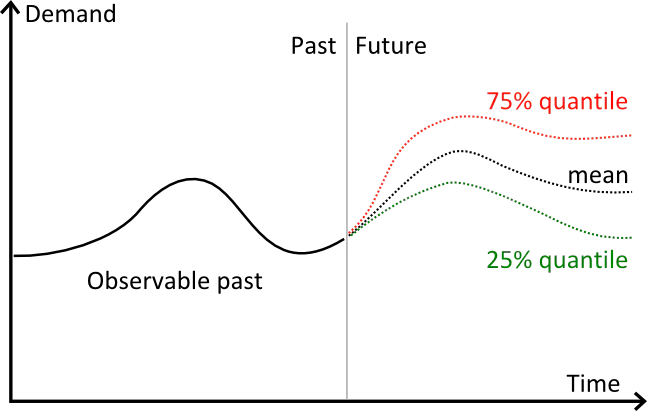
\includegraphics[width=0.8\textwidth]{capitulos/cap_02/imagenes/quantile_regression.png}
    \caption[
        Gráfico que ilustra las 3 predicciones que arroja un modelo de regresión cuantílica. Recuperado de 
        \cite{vermorel2012}.
    ]{
        Gráfico que ilustra las 3 predicciones que arroja un modelo de regresión cuantílica. Recuperado de 
        \cite{vermorel2012}. Se observa los límites superior e inferior los percentiles 75 y 25, 
        respectivamente. 
    }
    \label{fig:quantile_regression}
\end{figure}

Sin embargo, este método presenta varios problemas:

\begin{itemize}

    \item Sensibilidad a datos escasos o ruidosos: La estimación puede ser muy sensible a 
    \textit{outliers}
    \footnote{
        Los valores atípicos o \textit{outliers} son instancias que se desvían significativamente del resto
        de instancias del conjunto de datos. Un \textit{outlier} podría indicar un comportamiento anormal
        del sistema (variabilidad natural del fenómeno observado, eventos excepcionales que refleja 
        comportamientos reales pero poco frecuentes, ...) o un error de recolección y registro de los datos 
        \cite{alpaydin2010}.   
    } 
    y a regiones con pocas observaciones, llevando a intervalos poco fiables. De hecho, se puede dar el 
    fenómeno indeseable de que cuantiles mayores tengan valores predichos más bajos que cuantiles menores 
    ---conocido como cruzamiento de cuantiles \cite{koenker2005}---.
    
    \item Falta de cobertura probabilística garantizada: No existe ningún tipo de garantía estadística que 
    asegure que el cuantil estimado cubra la proporción deseada de observaciones en muestras futuras. 
    
    \item No captura la incertidumbre epistémica: Solo captura la incertidumbre aleatoria \cite{abdar2021},
    dado que modela cómo los valores de salida varían dado un conjunto de entradas. No captura automáticamente 
    incertidumbre epistémica, a menos que se combine con otros enfoques, como métodos bayesianos 
    \cite{tokdar2012}.

    \item Muestran gran incertidumbre en cuantiles extremos (cerca de cero o uno) \cite{feldman2023} y, por 
    tanto, los intervalos de predicción obtenidos son extremedamente grandes, lo que logra una gran cobertura
    pero poca utilidad práctica. 
    
\end{itemize}


Otra técnica que no ...


\todo{Introducir la predicción conformal}



\subsubsection{Cuantificación de la incertidumbre en problemas de clasificación}



\todo{¿Introducir la calibración de modelos y centrarse en el Platt Scaling y Temperature Scaling?}


\todo{Introducir la predicción conformal}



% ------------------------------------------------------------------------------------------------------------
% CONFORMAL PREDICTION ---------------------------------------------------------------------------------------
% ------------------------------------------------------------------------------------------------------------

\section{Conformal Prediction}

La \textbf{predicción conformal (\textit{conformal predition}, CP)} 

% ------------------------------------------------------------------------------------------------------------

\subsection{Conformal Prediction en problemas de regresión}

\subsubsection{Conformalized Quantile Regression (CQR)}


\subsubsection{}



% ------------------------------------------------------------------------------------------------------------

\subsection{Conformal Prediction en problemas de clasificación}

...

\begin{figure}[h]
    \centering
    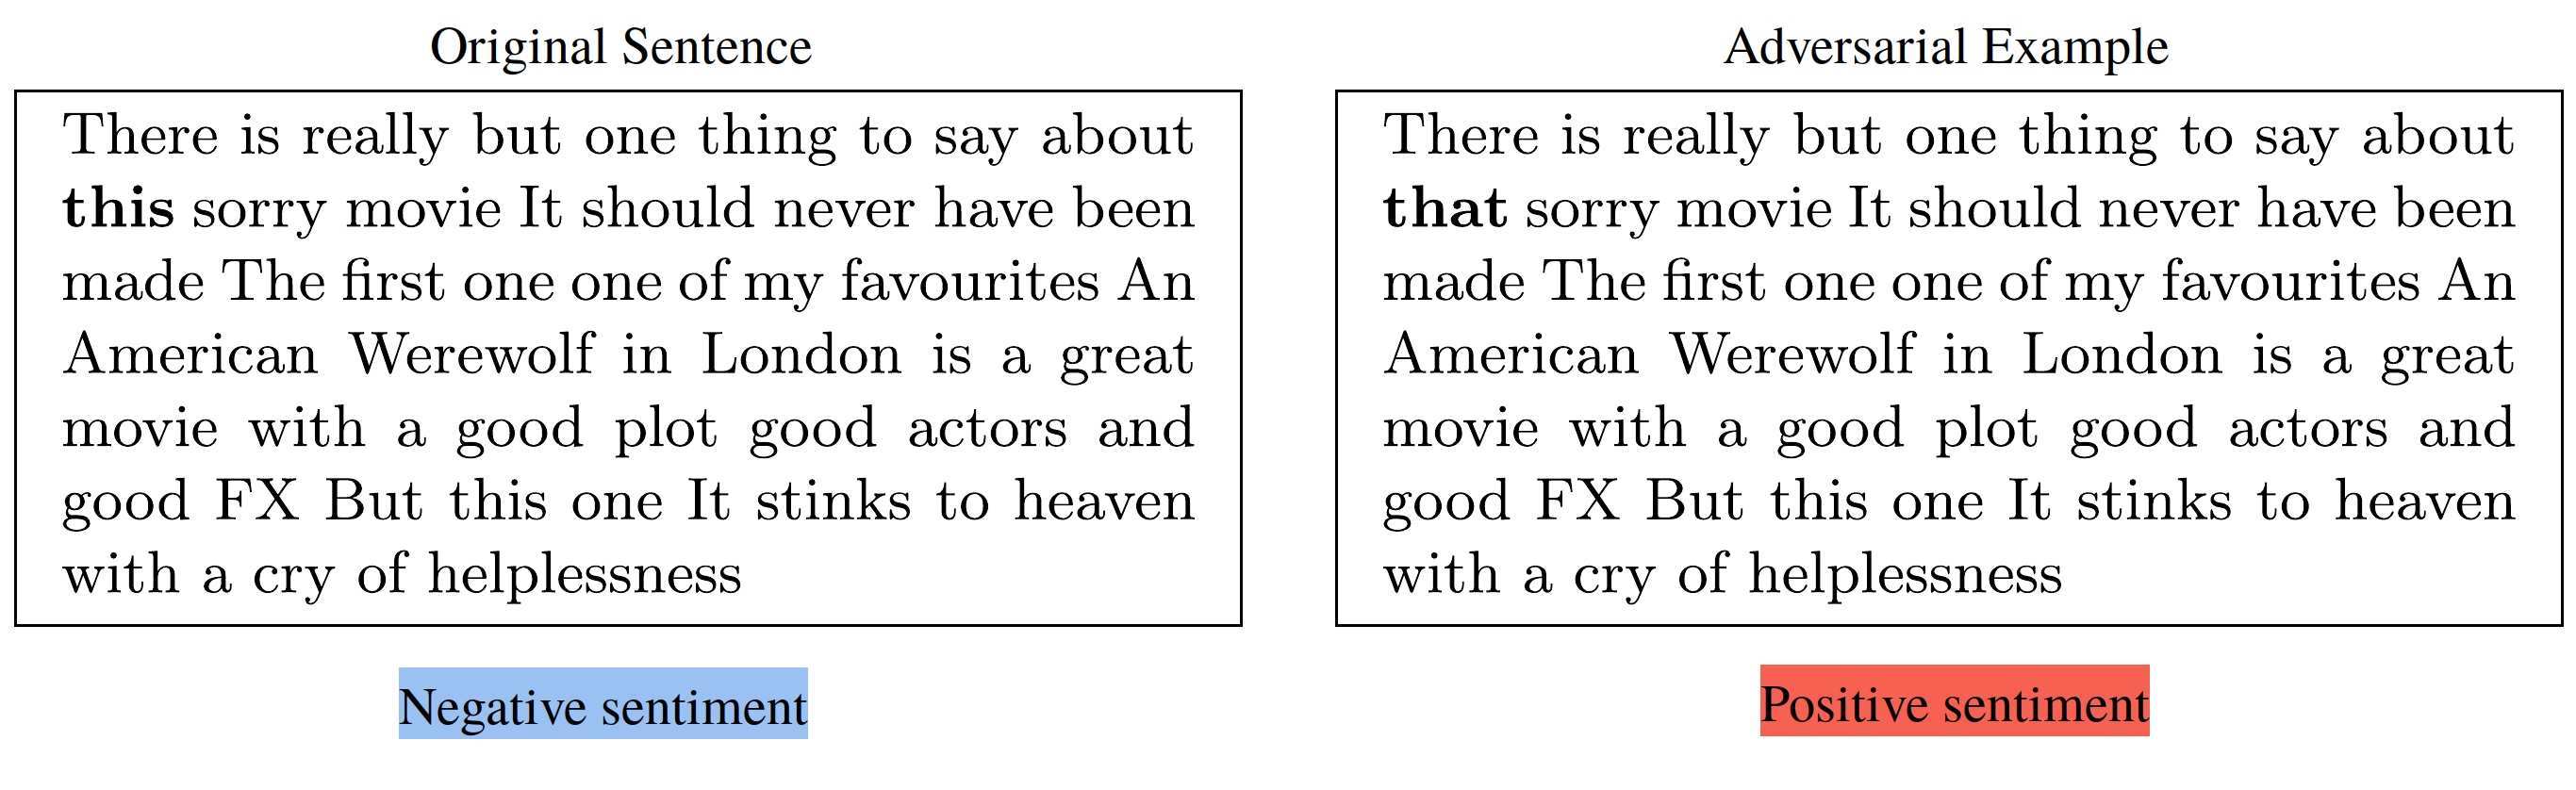
\includegraphics[width=\textwidth]{capitulos/cap_02/imagenes/adversarial_example.png}
    \caption[
        Ejemplo adverario mal clasificado por un modelo ML entrenado con datos textuales.
        Adaptado de la Figura 2 de \cite{hullermeier2021}, original de \cite{sato2018}.
    ]{
        Ejemplo adverario mal clasificado por un modelo ML entrenado con datos textuales.
        Adaptado de la Figura 2 de \cite{hullermeier2021}, original de \cite{sato2018}.
        Se observa que el cambio de una sola palabra ---y aparentemente sin mucha relevancia--- (destacada en 
        negrita) basta para cambiar la predicción de ``sentimiento negativo'' a ``sentimiento positivo''.
    } 
    \label{fig:adversarial_example}
\end{figure}

\subsubsection{Least-Ambiguous Set-Valued Classifiers}

...

\subsubsection{Adaptive Prediction Sets}

El \textbf{\textit{Adaptive Prediction Sets} (APS)} \cite{romano2020}

\subsubsection{Regularized Adaptive Prediction Sets}

\textbf{\textit{Regularized Adaptive Prediction Sets} (RAPS)} \cite{angelopoulos2020} es una variante del método APS, 
que 

añade una penalización a conjuntos de predicción demasiado grandes, realizando esto a través 
de la suma de un componente 




